%Project Report for CS296 : Software Systems Lab
%Created by Group 2

%Document Class
\documentclass[a4paper,11pt]{article}

%Packages Used
\usepackage[top=1in, bottom=1in, left=0.5in, right=0.5in]{geometry}
\usepackage{graphicx}
\usepackage{subfig}

%Document Starts Here
\begin{document}

%Information about the file
\title{\textbf{Sliding Gate: A CS296 Group 02 Report}}

\author{
Kshitij Singh\\
110050016\\
kkshitijs@cse.iitb.ac.in
\and
Prithviraj Madhukar Billa\\
110050065\\
prithvirajbilla@cse.iitb.ac.in
\and
Sahil Jindal\\
110020043\\
sahil@cse.iitb.ac.in
}

\date{\today}
\maketitle

\setlength{\parindent}{0 cm}
%Sections start here
\section{Introduction}

We have designed a machine that goes through a sequence of processes to end up performing a simple task - "Sliding a Gate". A pendulum starts off by toppling dominos that roll a ball on a pulley that enables a see-saw to throw a ball on unstable dominos that goes through a sequence of see-saws and hinges that ends up sliding a gate. Of course, you may ask why not just slide the gate? But that is just what a Rude Goldberg Machine is. As per Wikipedia,

A Rube Goldberg machine is a deliberately over-engineered or overdone machine that performs a very simple task in a very complex fashion, usually including a chain reaction. 

\section{Origin}

It all started way back in January 2013 when we had to first think of a design to implement as a course project. We were naive back then and thought of making a complicated machine. A sequence of processes will lead to a final goal, which we set as "Putting Out A Fire". The initially proposed design looked like this.

\begin{center}
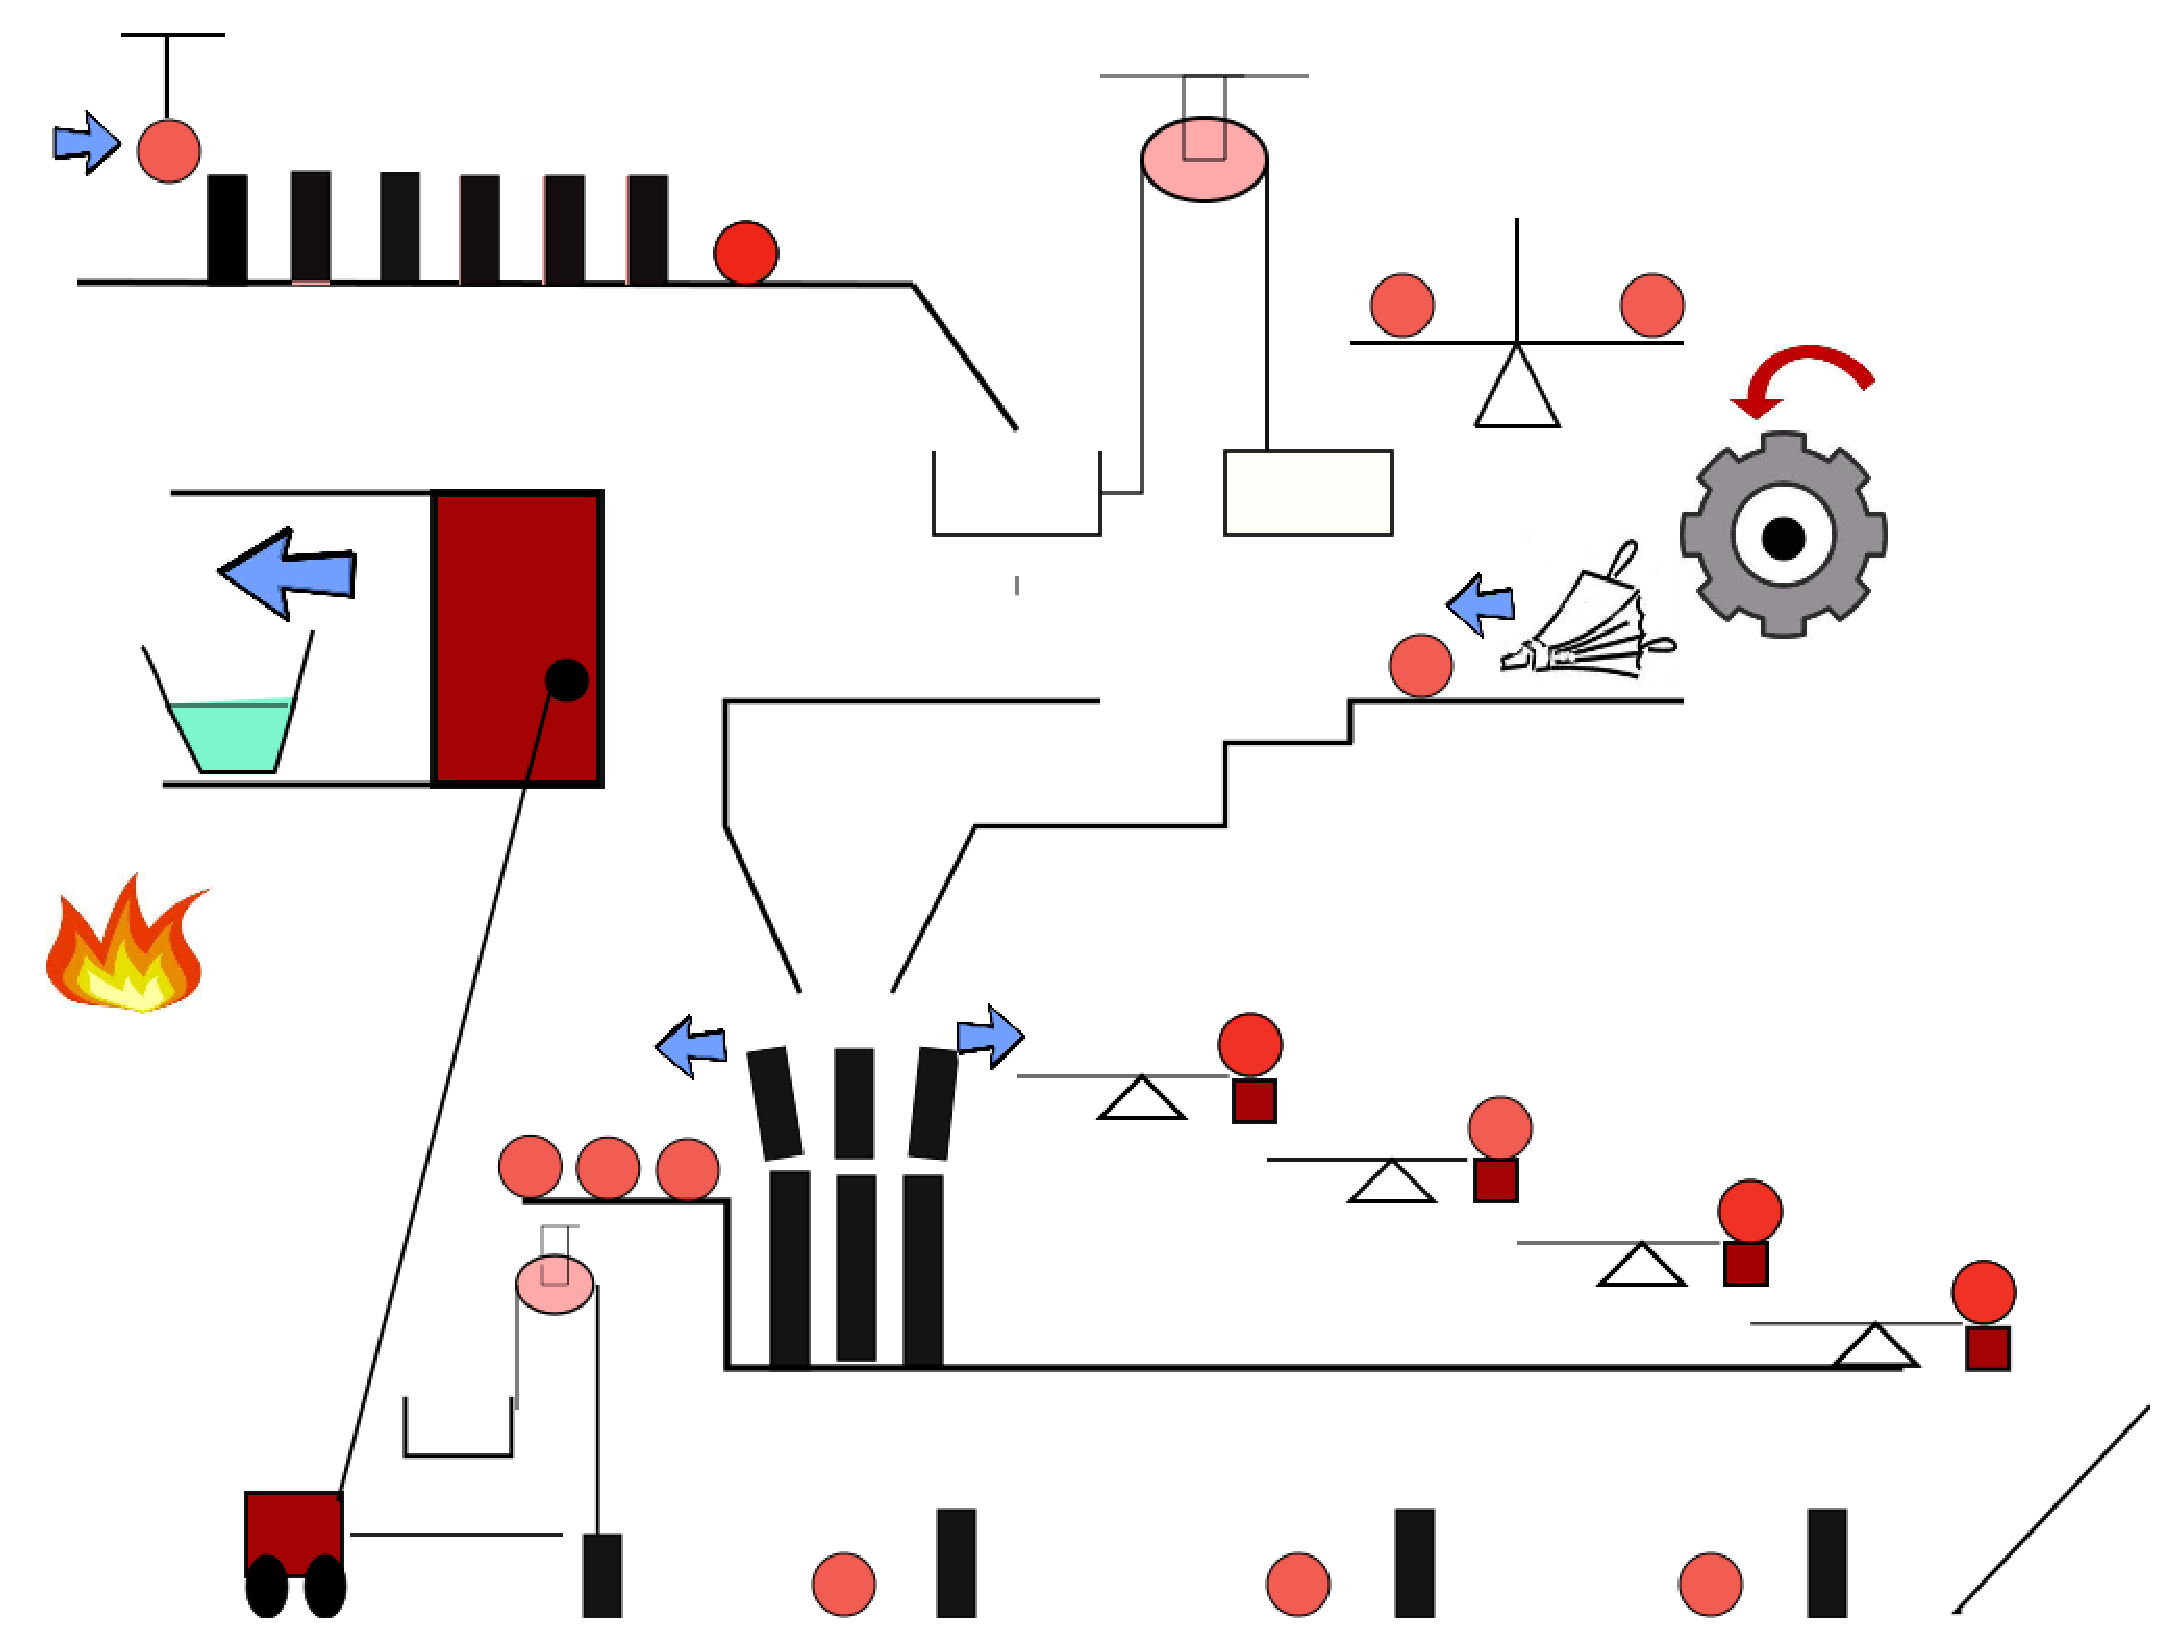
\includegraphics[width=180mm, height=120mm]{RubeGoldberg.eps}\\
\label{Fig. : Original Proposed Design of Rube Goldberg}
\end{center}

Of course, as we later found out, there were a few changes that had to be made in the design to adapt it to the Box2D environment. More on that in the next section.

\section{The Present State}

Currently, our design looks slightly different. A snapshot of the initial state is given below.

\begin{center}
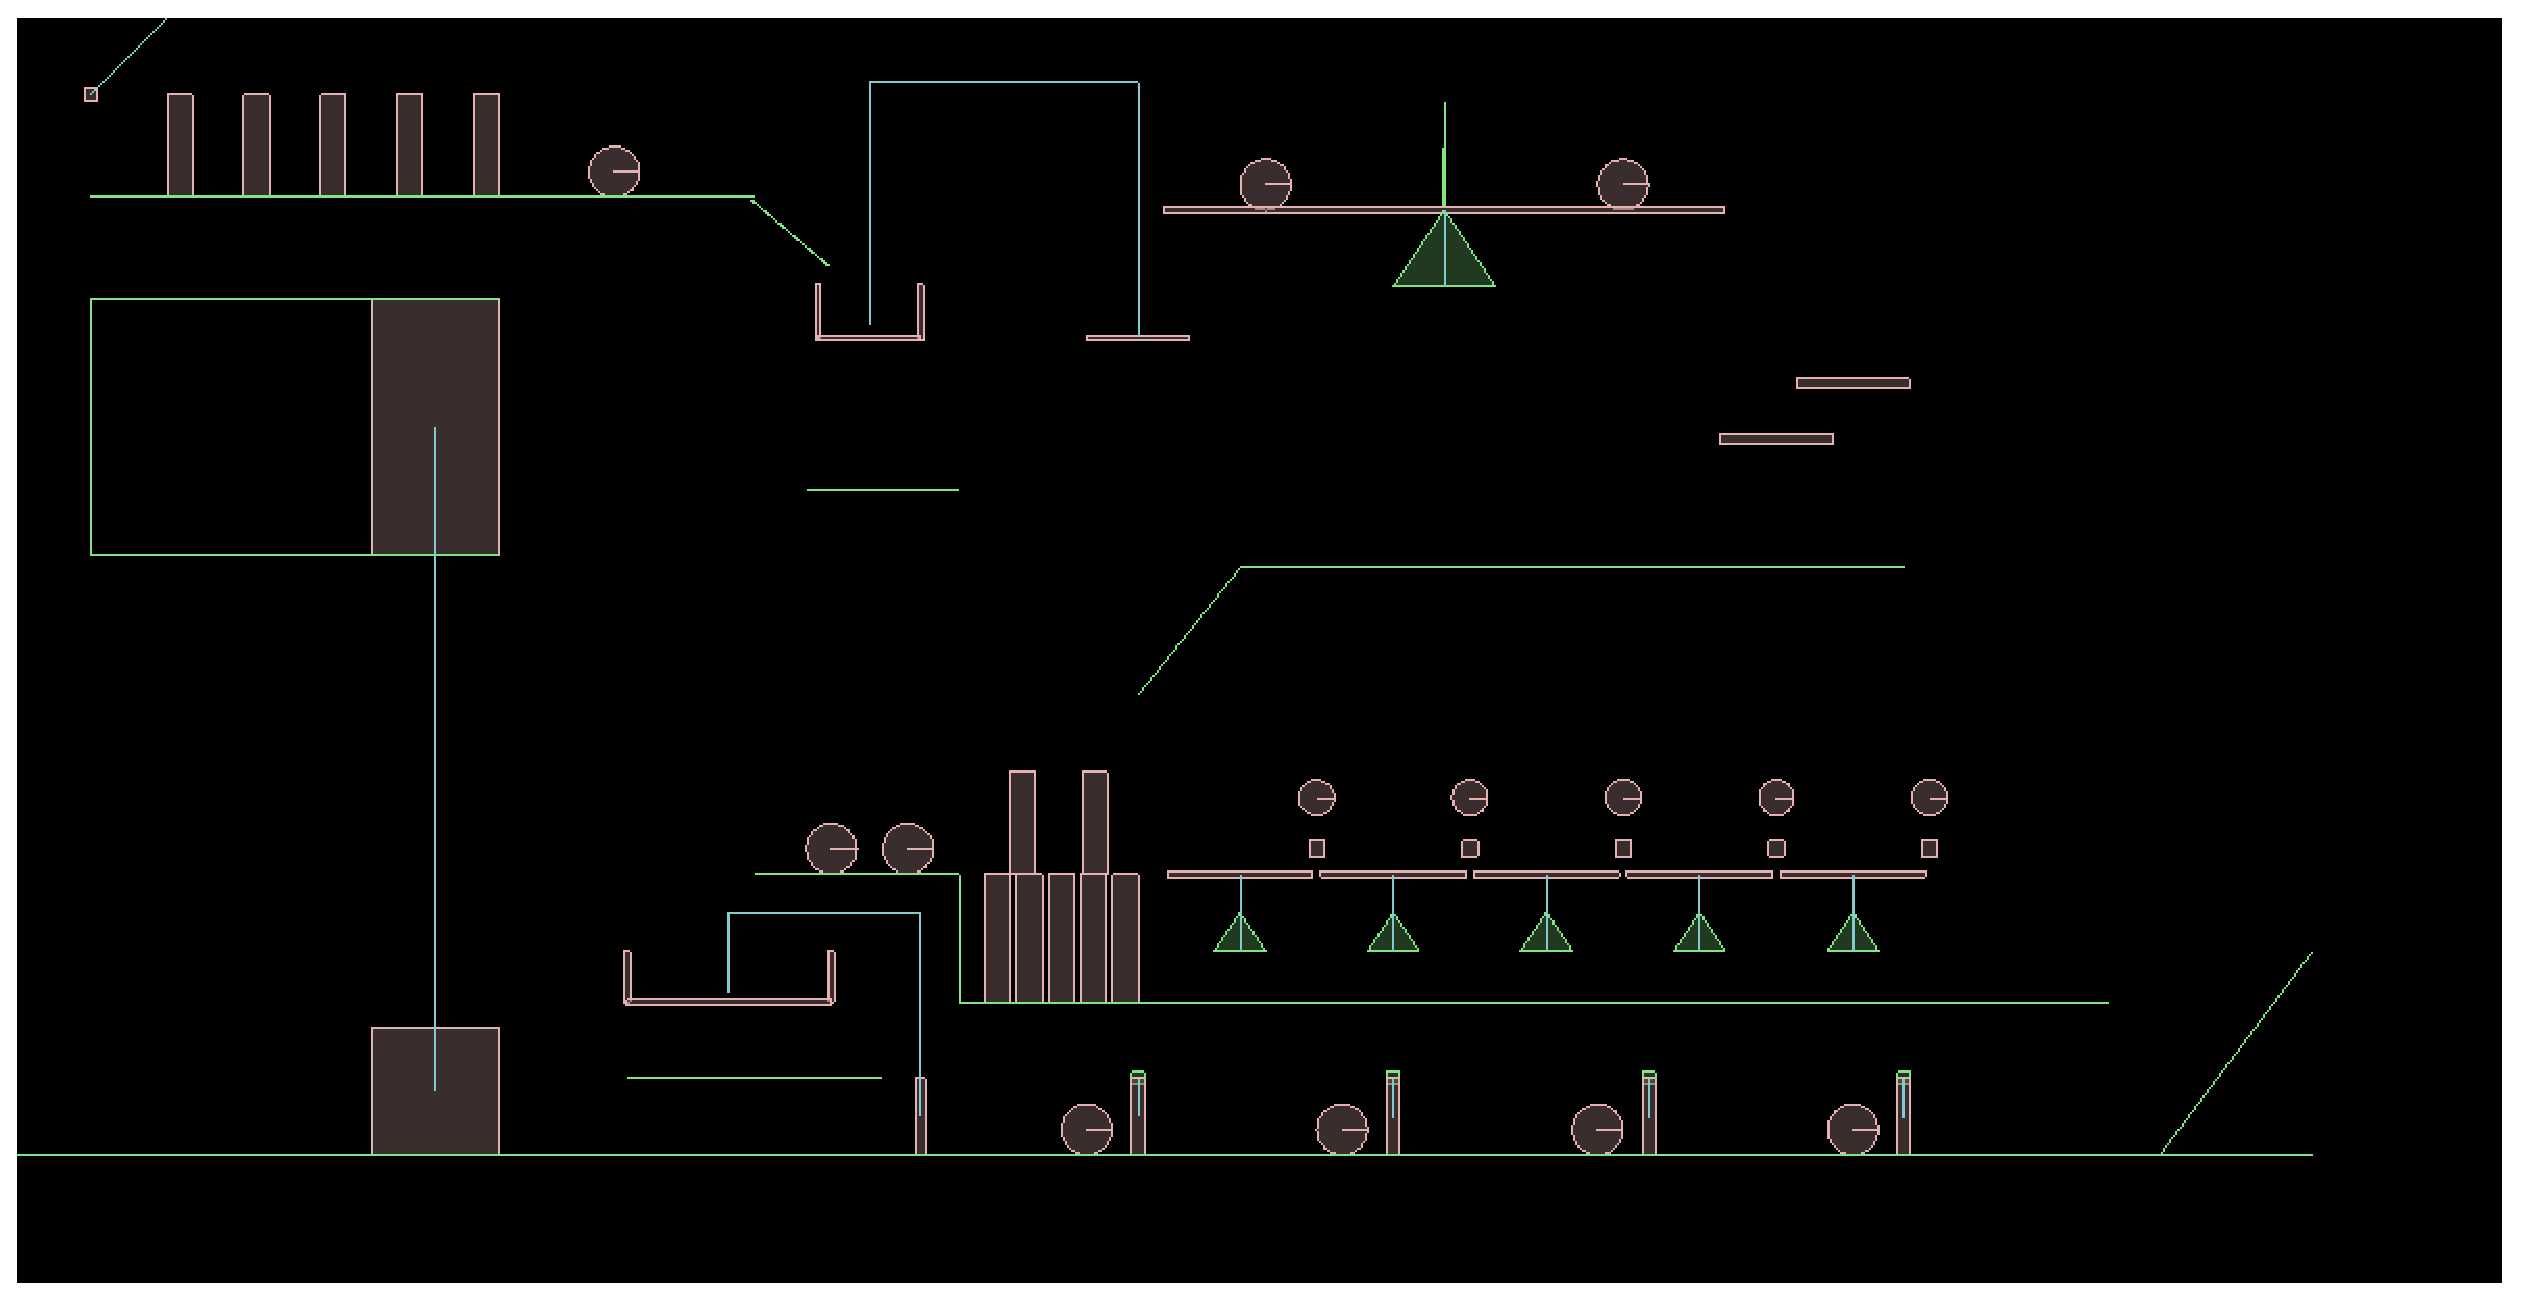
\includegraphics[width=160mm, height=120mm]{state_00.eps}\\
\label{Fig. : State of Machine before Start}
\end{center}

The machine includes the following elements:

\begin{itemize}

\item Pendulum 
\begin{itemize}
\item It knocks off dominos to start the simulation
\end{itemize}
\item Dominos system
\begin{itemize}
\item It topples onto a ball to set it rolling
\end{itemize}
\item A balanced pulley system
\begin{itemize}
\item It triggers a see-saw motion when unbalanced
\end{itemize}
\item See-Saw
\begin{itemize}
\item It drops a ball on a rotating platform
\end{itemize}
\item Rotating Platform
\begin{itemize}
\item It works as a gear substitute to give direction to the dropped ball
\end{itemize}
\item Unstable Dominos
\begin{itemize}
\item It is a shaky system that when triggered, sparks off two simultaneous processes
\end{itemize}
\item Linked See-Saws
\begin{itemize}
\item One see-saw triggers another, which leads finally to a ball falling down
\end{itemize}
\item Hinged Bars and Balls
\begin{itemize}
\item This works as a self-triggering system that finally leads to a ball speeding along the ground
\end{itemize}
\item Pulley-Gate System
\begin{itemize}
\item Here, the application of weight on the pulley leads to the raising of a gate
\end{itemize}
\item Sliding-Gate
\begin{itemize}
\item The final item that leads to a gate sliding along its frame
\end{itemize}

\end{itemize}

This brings us to the question what makes this design interesting. Read on!

\section{Unique is Interesting}

Unique things are quite interesting, aren't they? Well, here is some the interesting stuff about our design:

\begin {itemize}
\item The \emph{Linked See-Saw} system is a nice element in the design. Here the ball from one see-saw falls on a neighbouring see-saw which happens till 4 steps finally leading to a ball rolling off. This is quite elegant and is definitely one of the high-points of the simulation.
\item Another one is the \emph{Hinged Bars and Balls} system which, thanks to the manipulation of densities of the bar and the ball, leads the observer to the illusion that energy is being created. The balls suddenly seem to pick up speed. Obviously, no external force is given at this stage and it creates an interesting thing to watch. Also, it helps us later since the speed is needed to slide the gate.
\item The \emph{Shaky Dominos} is a nice concept since it allows us to break a sequential process into two sequential processes that heppen simultaneously. The dominos have been arranged such that one of them falls to the left leading to some processes, while the other one falls to the right simultaneously triggering the linked see-saws.
\item We personally prefer the \emph{Sliding Gate}. That has been created by putting a rectangular body among frames, and then connecting it through a \emph{Distance Joint} with a \emph{denser} body kept below on the ground. The movement of that body leads to the final sliding of the gate.
\end{itemize}

The machine required some fine-tuning. That involves routine stuff like positioning elements correctly and triggering them at the right time. But there are a few points that we would like to bring to the notice.

\subsection{The Gear Hack}

This was done to substitute the gear that was proposed in the original design. The gear was basically needed just to change the direction of the rolling ball. It seemed cumbersome to add the gear as earlier proposed in its image form. Rather, we decided to compromise on the visual appeal and instead have ended up with a bar hinged at its center. At the start a vertical bar falls on this bar to set it rotating.  When a ball falls on this now rotating bar, its direction is changed to where we want it to go. This is the same functionality that was required of the gear, and works just fine for our purposes. Also, it kind of looks cool.

\subsection{Fire Runs Cold}

As noted earlier, our objective was to put out a fire. While it did seem interesting at that time, it soon started to seem a stupid thing to do with a Rube Goldberg Machine. Over time, this final objective underwent many changes. Initially, two images were needed - those of a pail of water and a raging fire. This basically involved falling of a body on another. Now, at the end, the objective has been modified to a more logical and reasonable one - sliding of a gate. And, seriously, this looks way better than what we had initially in mind.

\section{Timing Analysis}

Timing analysis is a key part of any project. It is a good indicator of the efficiency of the written code. So, here we have generated 
different plots and present an analysis based on them.

\subsection{Results from the graphs generated}

\begin{itemize}
\item As the number of iterations increase , the average step time, average times for collisions, position and velocity updates all decrease. This is due to the fact when the number of iterations increase , some variables will not be re-computed in subsequent iterations.
As a result , the average times will go down.
\item As the number of iterations increase , the loop time also increases (first linearly upto about 30 iterations and then at a less than linear rate). This is so since it includes the time for collision resolution, position and velocity updates which decrease on incrementing the number of iteratios.
\item All times remain nearly same for different rerun values.This is very logical since just running the code again with same inputs should give similar times.
\item Graph 5 plots the histogram of frequency of different step time values for 16 iterations. There is no clear pattern but when there is heavy load, a bell shaped histogram is obtained.
\end{itemize}

\section{Profiling the Release-version}

The profiling was done here following these steps :

\begin{itemize}

\item We built the Box2D library in the \emph{Debug} version, using cmake \emph{-DCMAKE\_BUILD\_TYPE=Release ../}
\item The code was run for 2,00,000 iterations to generate the profile data. 
\item The optimisation flags \emph{-O3} were used before compiling and linking.

\end{itemize}

\subsection{Analyzing Flat-Profile}

The Release version itself includes optimizations in its build process. Plus, we have also included the optimisation flag \emph{-O3} in the compiling and linking process. This leads to highly efficient code, that runs almost \emph{6 times faster}. There is a listing of \emph{55} functions, of which the most intensive are $\approx 5-10$ only. 

\begin{center}
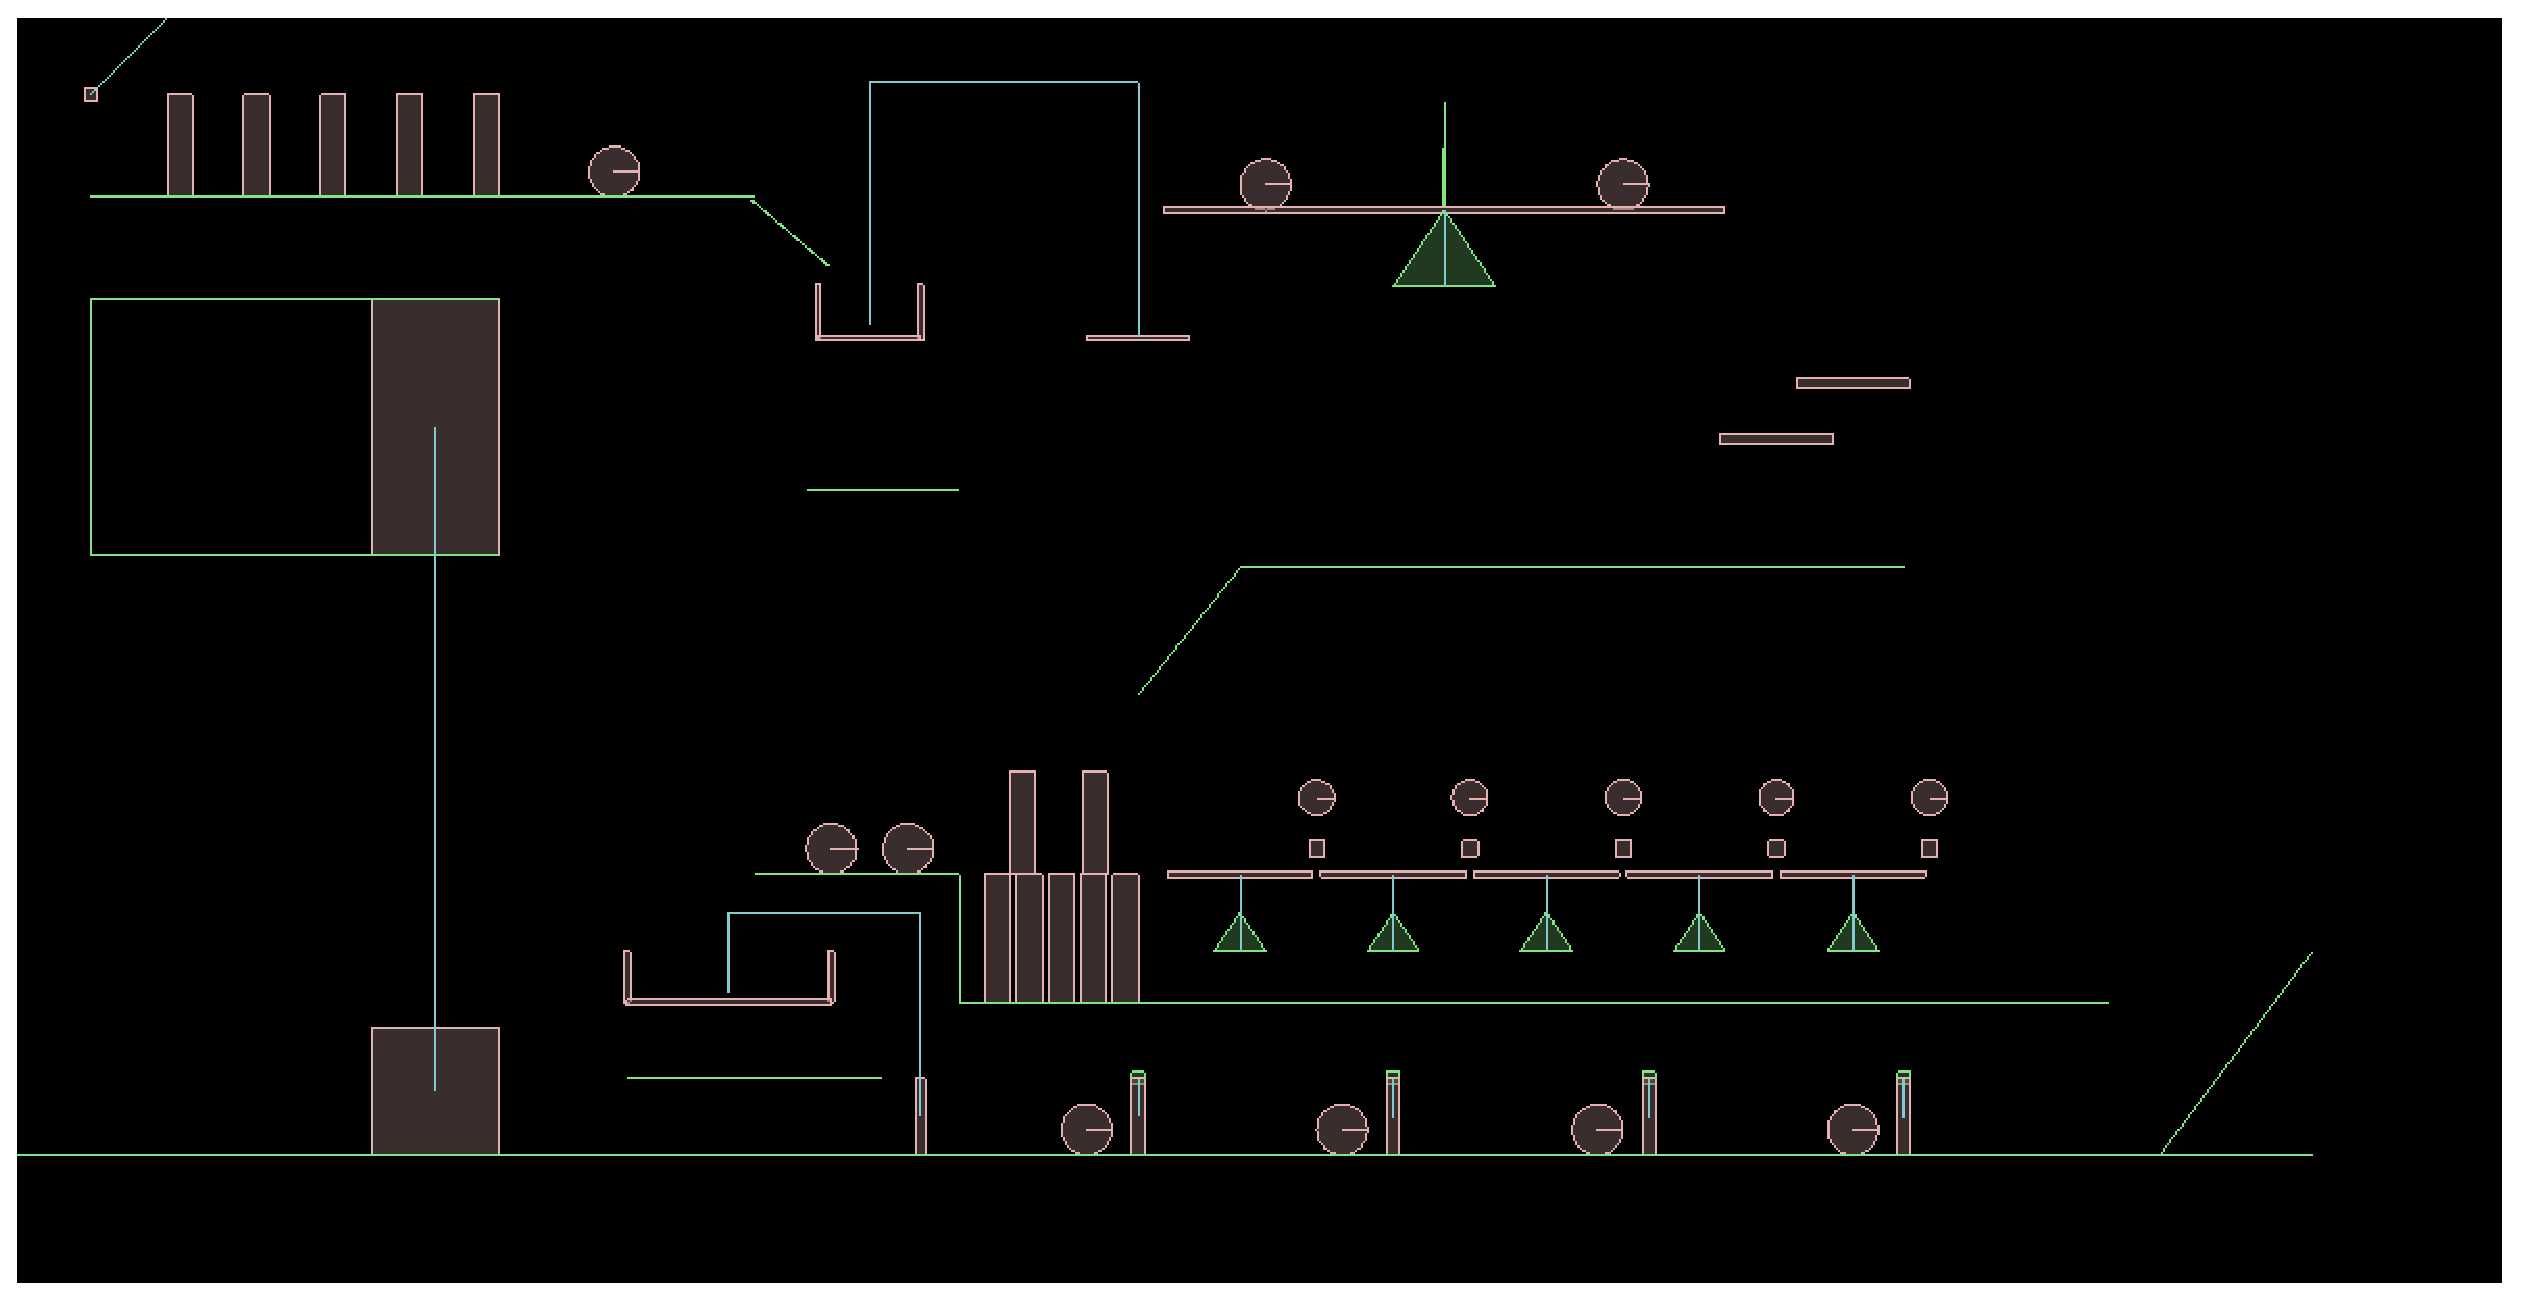
\includegraphics[width=195mm, height=60mm]{state_00.eps}\\
\emph{Fig. 3 : Flat Profile Data for Release-version profiling}
\end{center}

The following conclusions can be drawn from the flat profile data :

\begin{itemize}

\item Total time taken by the functions : \emph{5.07 seconds}
\item Most intensive functions : 
\begin{itemize}
\item \emph{b2ContactSolver::SolveVelocityConstraints()}
\item \emph{b2ContactSolver::SolvePositionConstraints()}
\end{itemize}
\item Time taken by most intensive functions : 
\begin{itemize}
\item \emph{b2ContactSolver::SolveVelocityConstraints()} : \emph{2.36 seconds}
\item \emph{b2ContactSolver::SolvePositionConstraints()} : \emph{0.31 seconds}
\end{itemize}

\end{itemize}

\subsection{Analyzing Call-Graph}

The call graph for the Release-version profiling is totally horizontal, indicating that the child functions have been placed \emph{inline}. This is just the optimisations that we had talked about in the earlier section. This turns out to be quite an efficient implementation, since it removes all the interconnections between the different functions, and leads to a highly structured and layered function call pattern.

\begin{center}
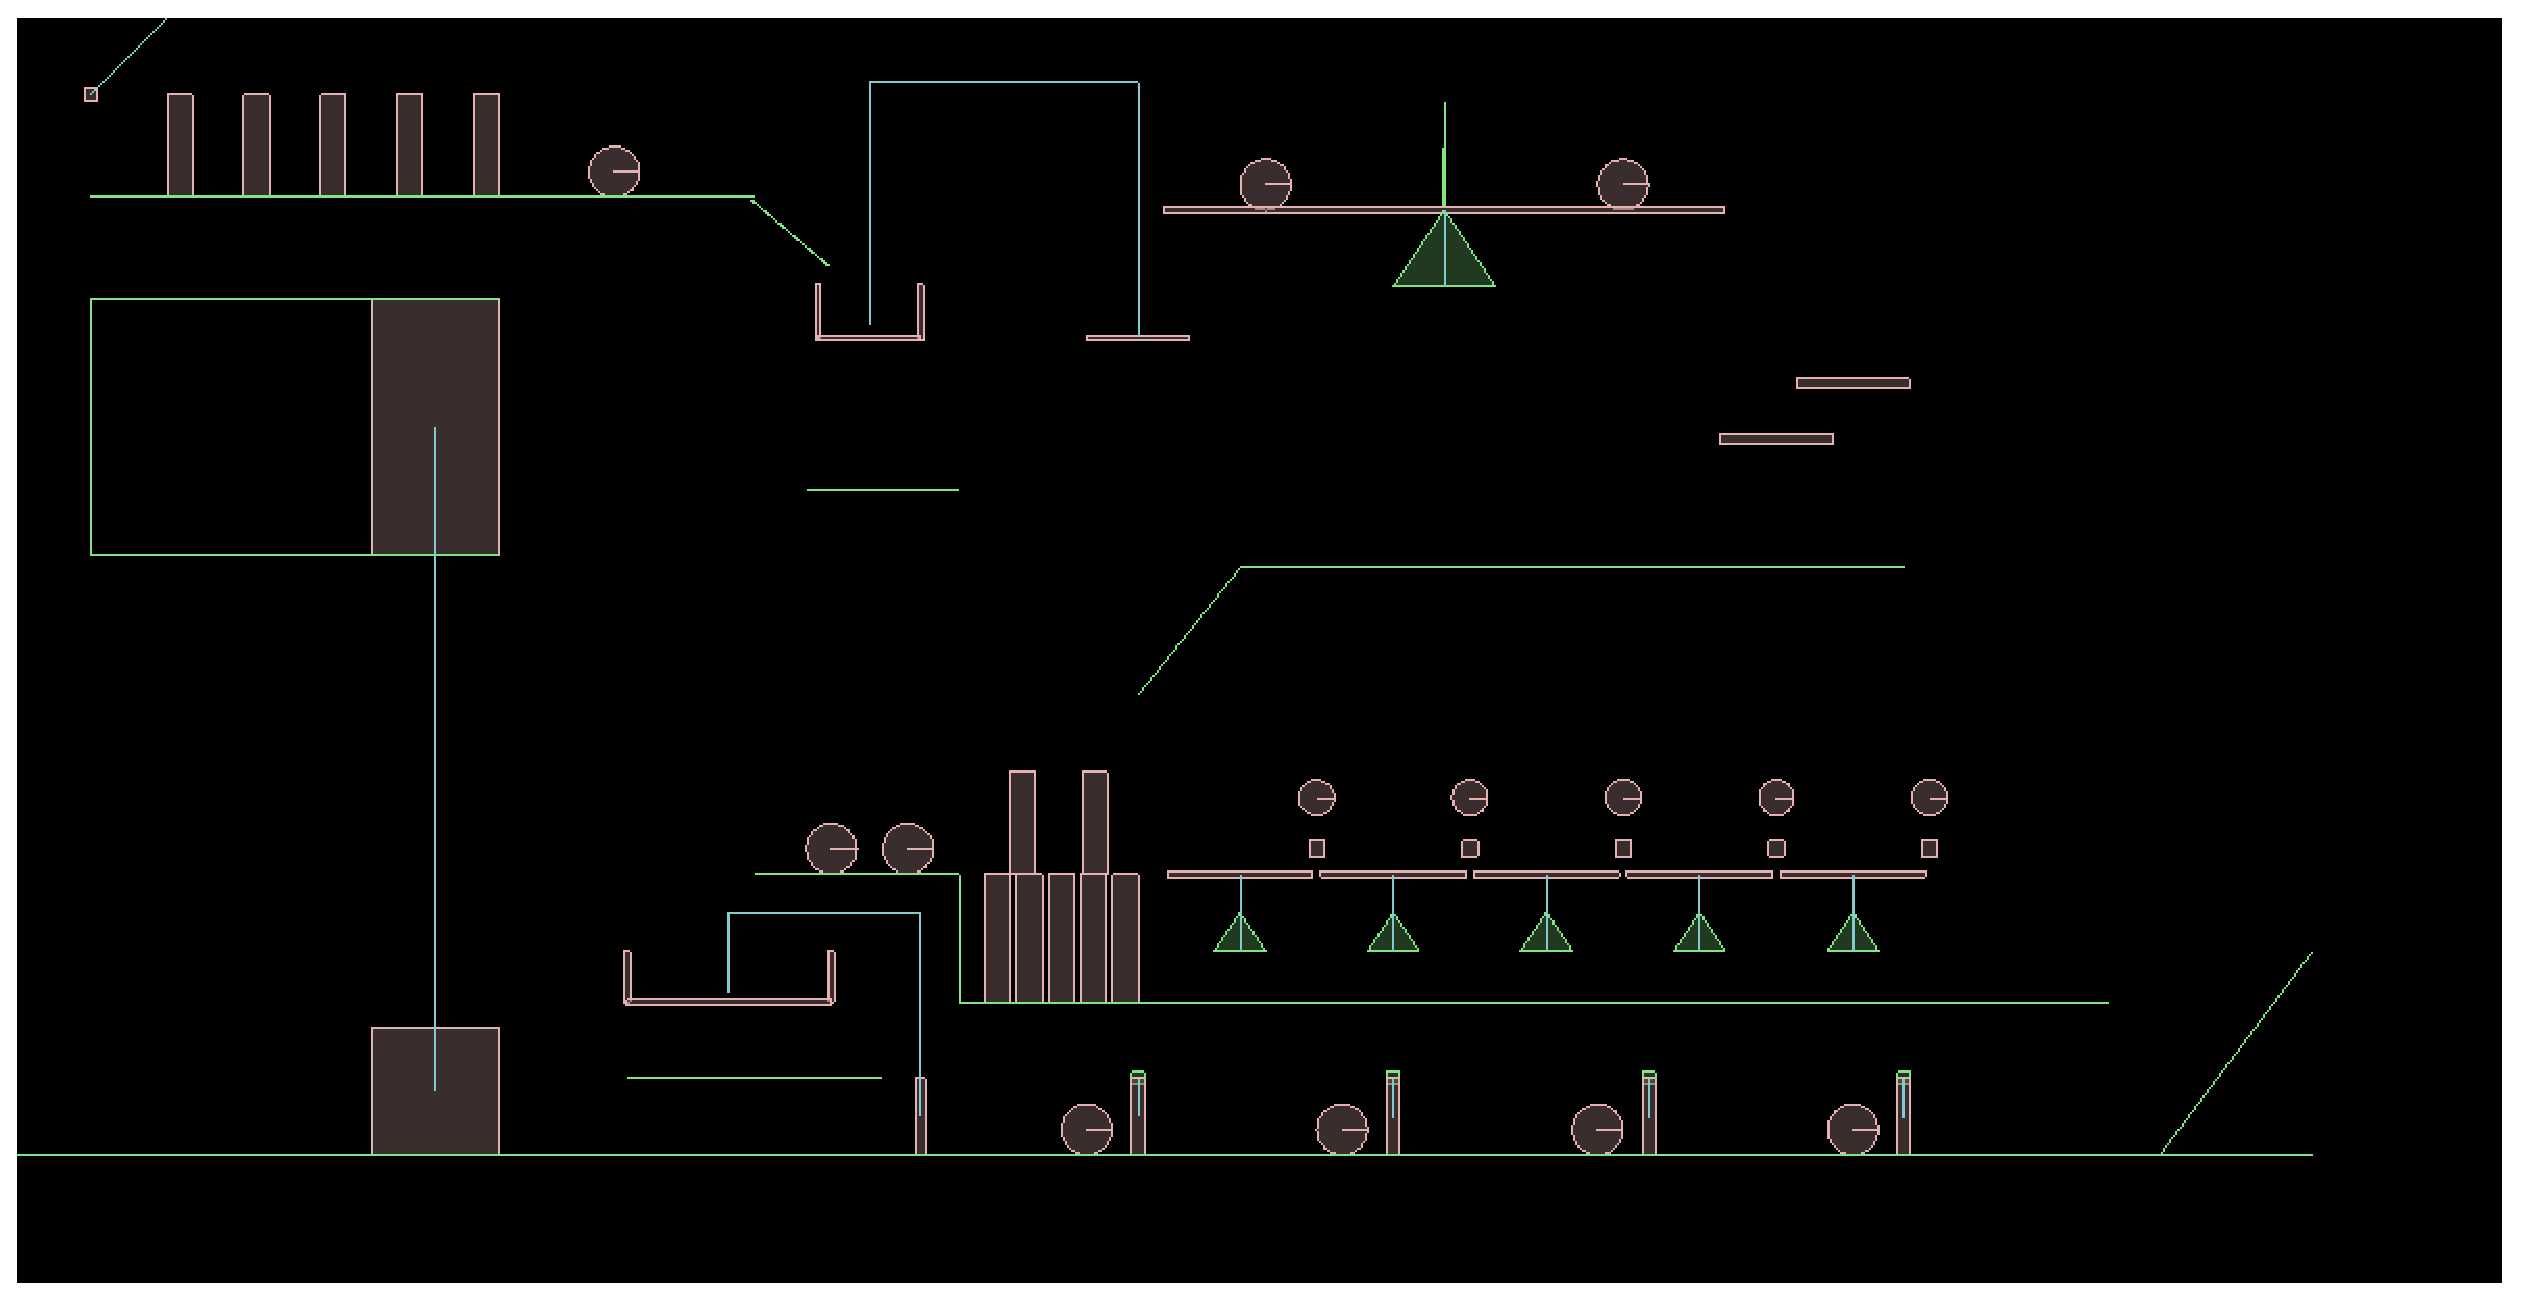
\includegraphics[width=195mm, height=30mm]{state_00.eps}\\
\emph{Fig. 4 : Cropped Call Graph for Release-version profiling}
\end{center}





\section{A Thousand Words}

Here we present the snapshots of the Rube Goldberg Design at its various stages.

\begin{figure}
\centering
\subfloat[Fig. : Stage 1]{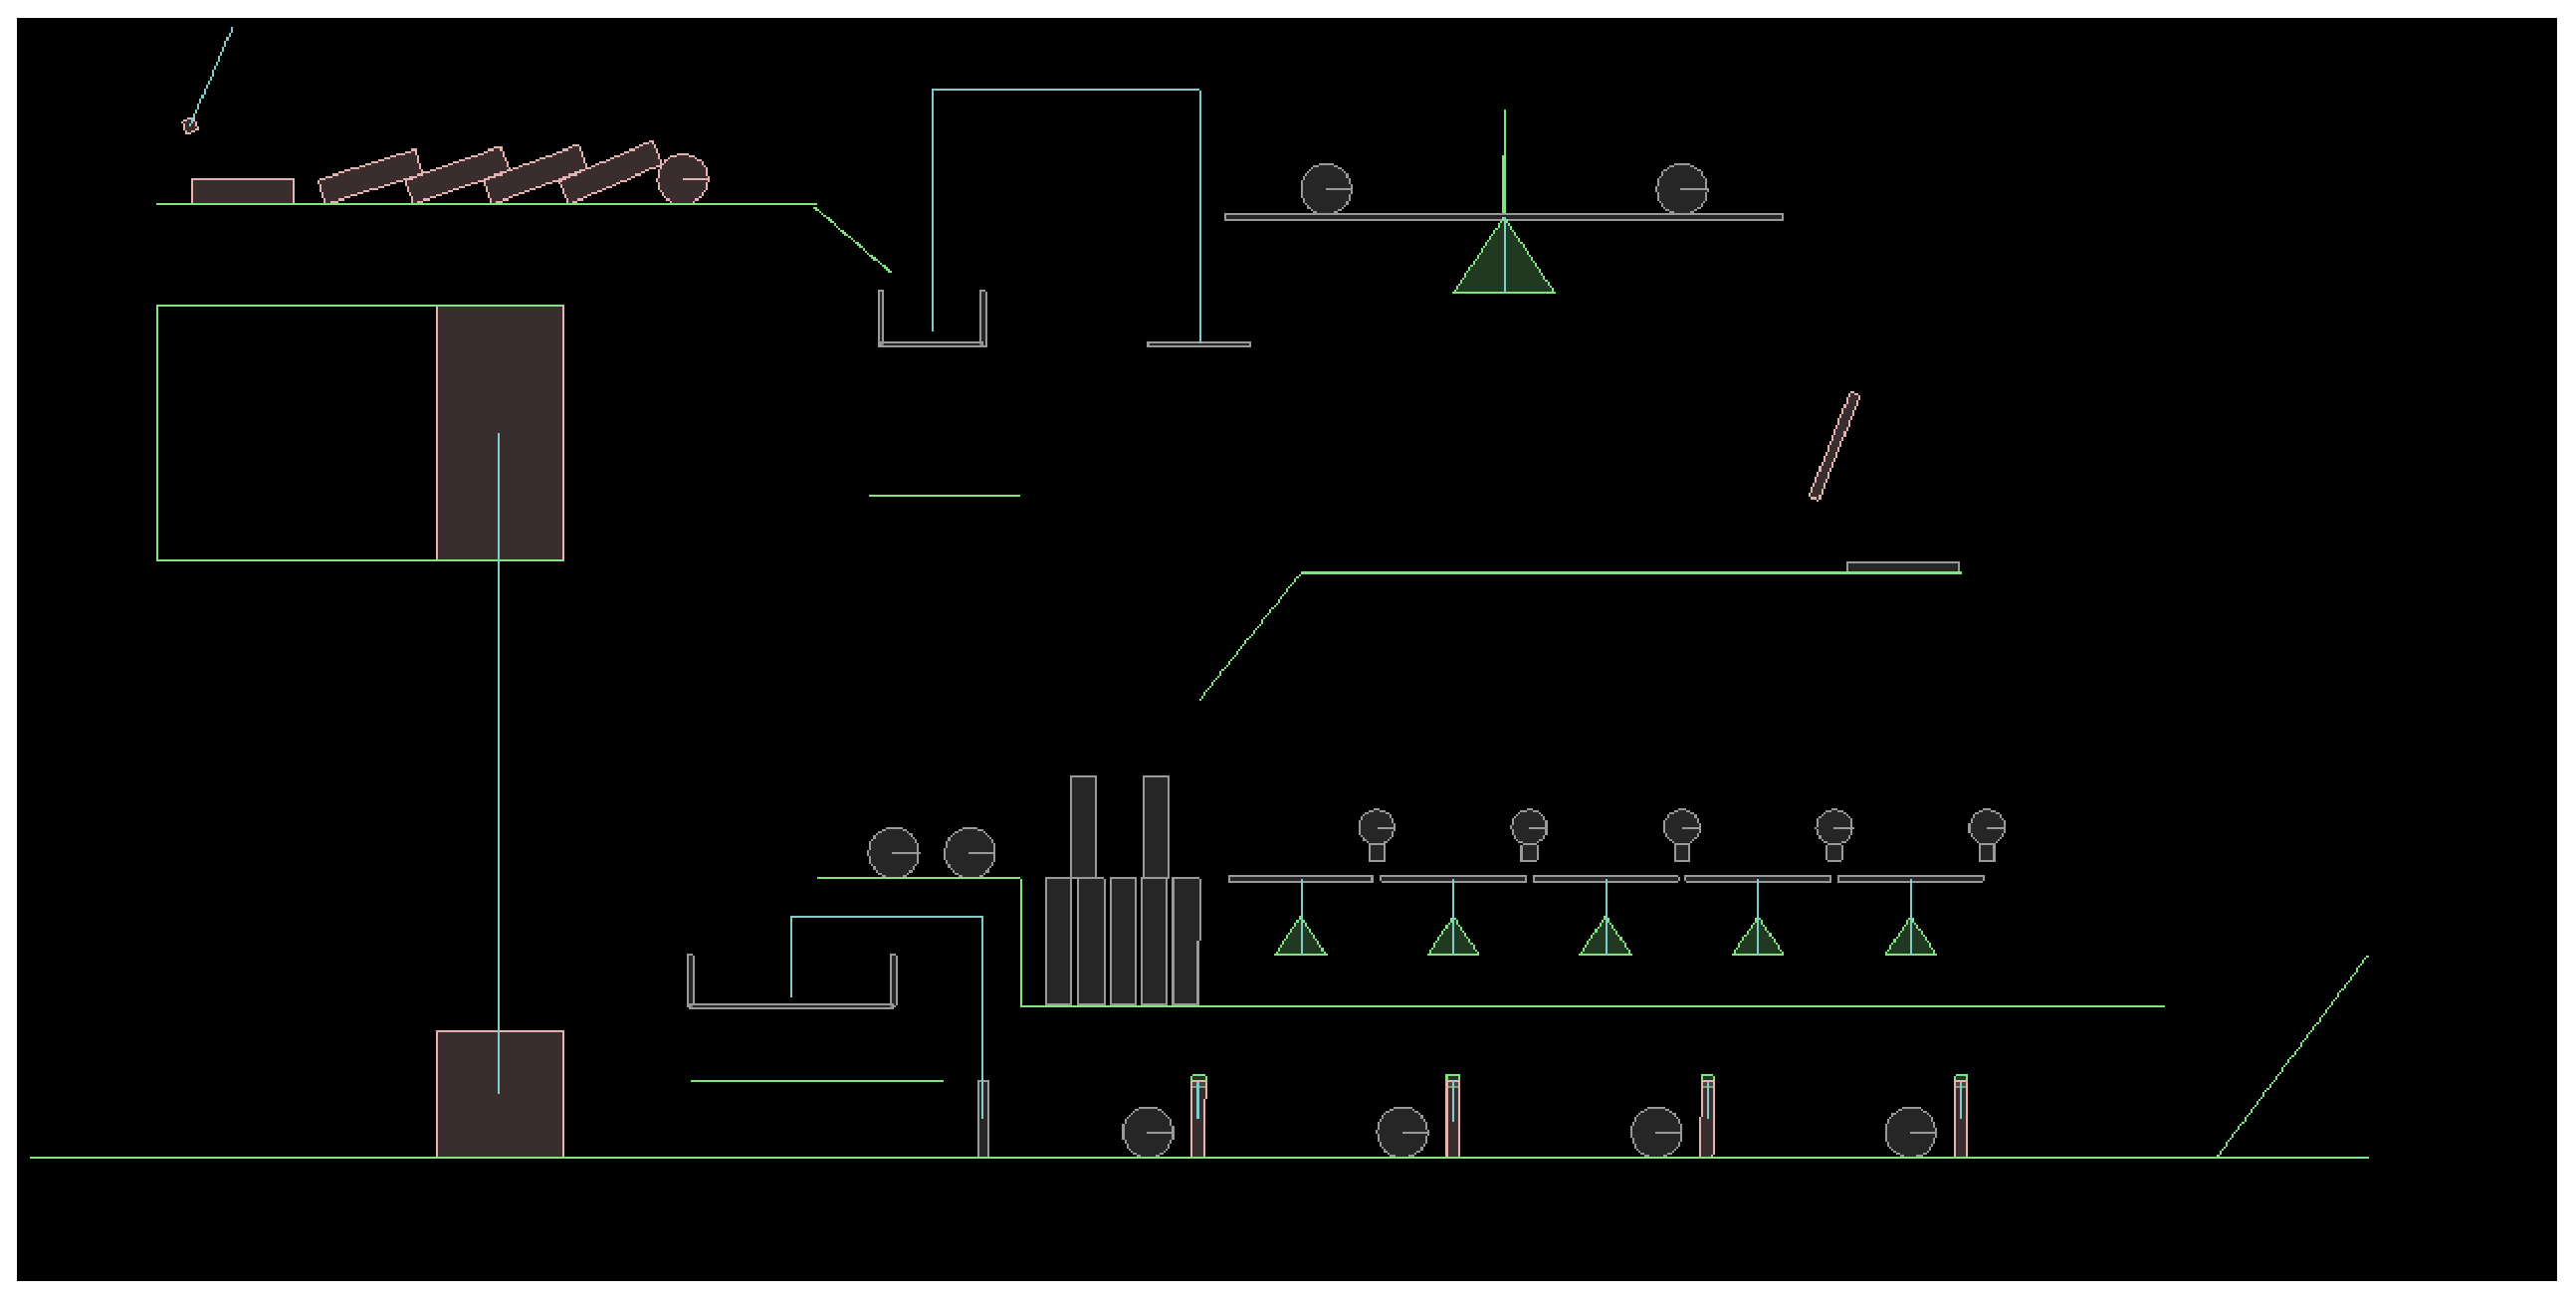
\includegraphics[width=70mm, height=50mm]{state_01.eps}}
\subfloat[Fig. : Stage 2]{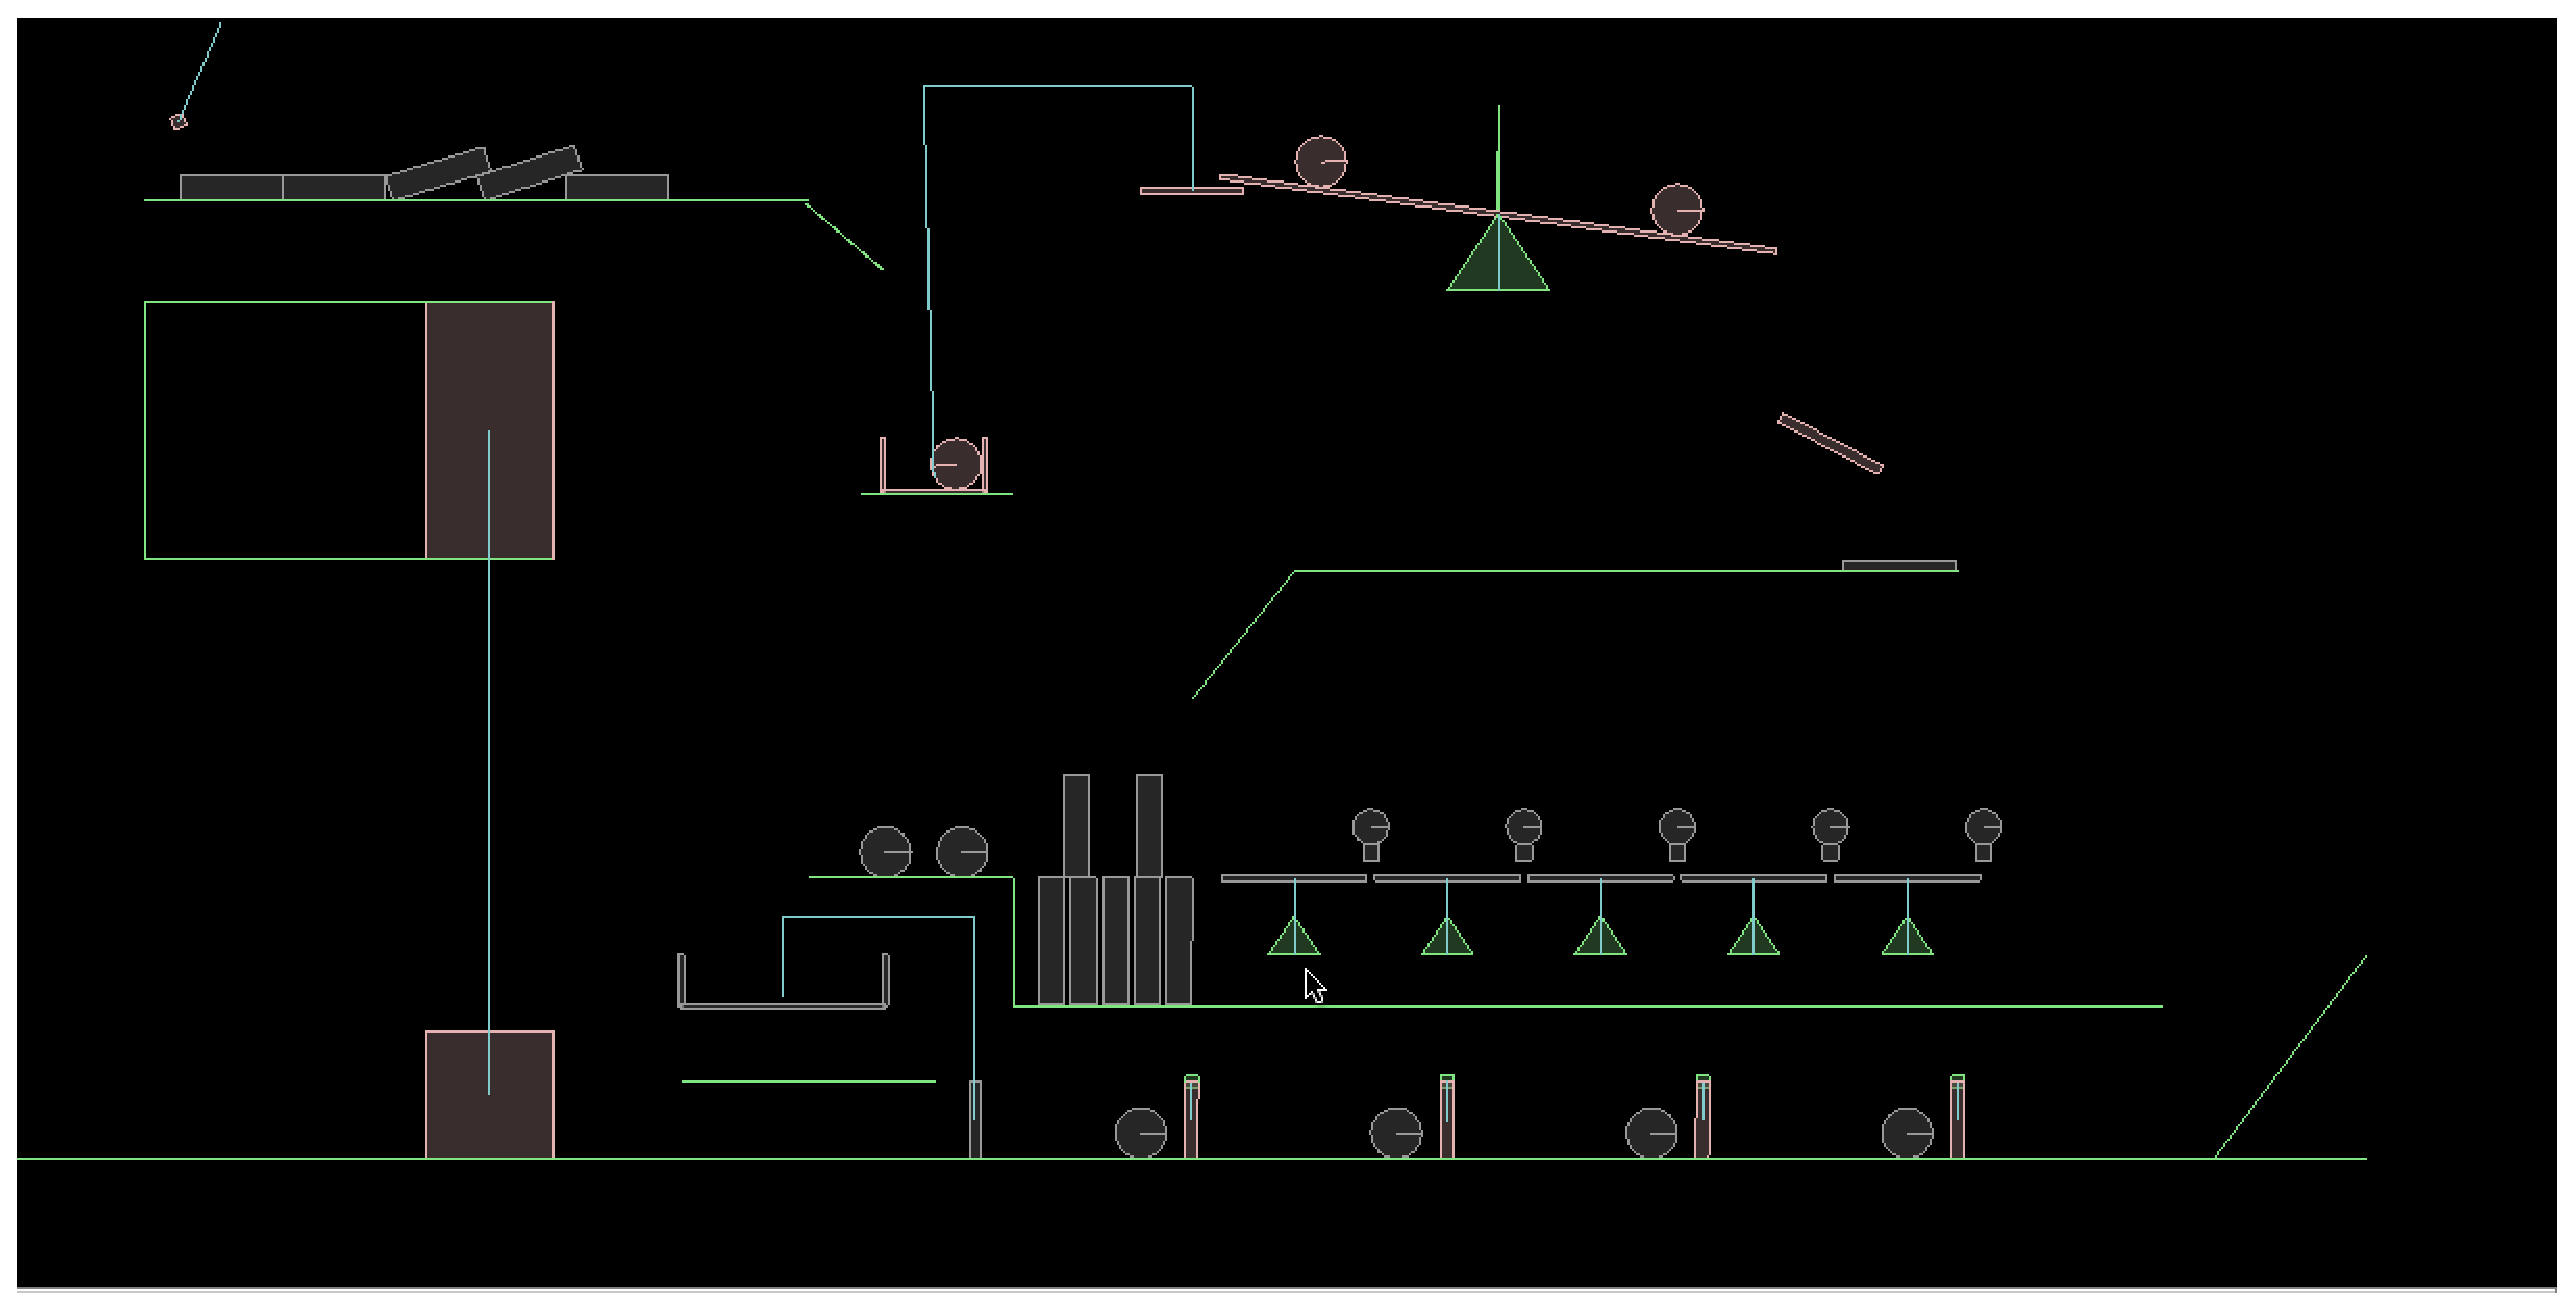
\includegraphics[width=70mm, height=50mm]{state_02.eps}}\\
\subfloat[Fig. : Stage 3]{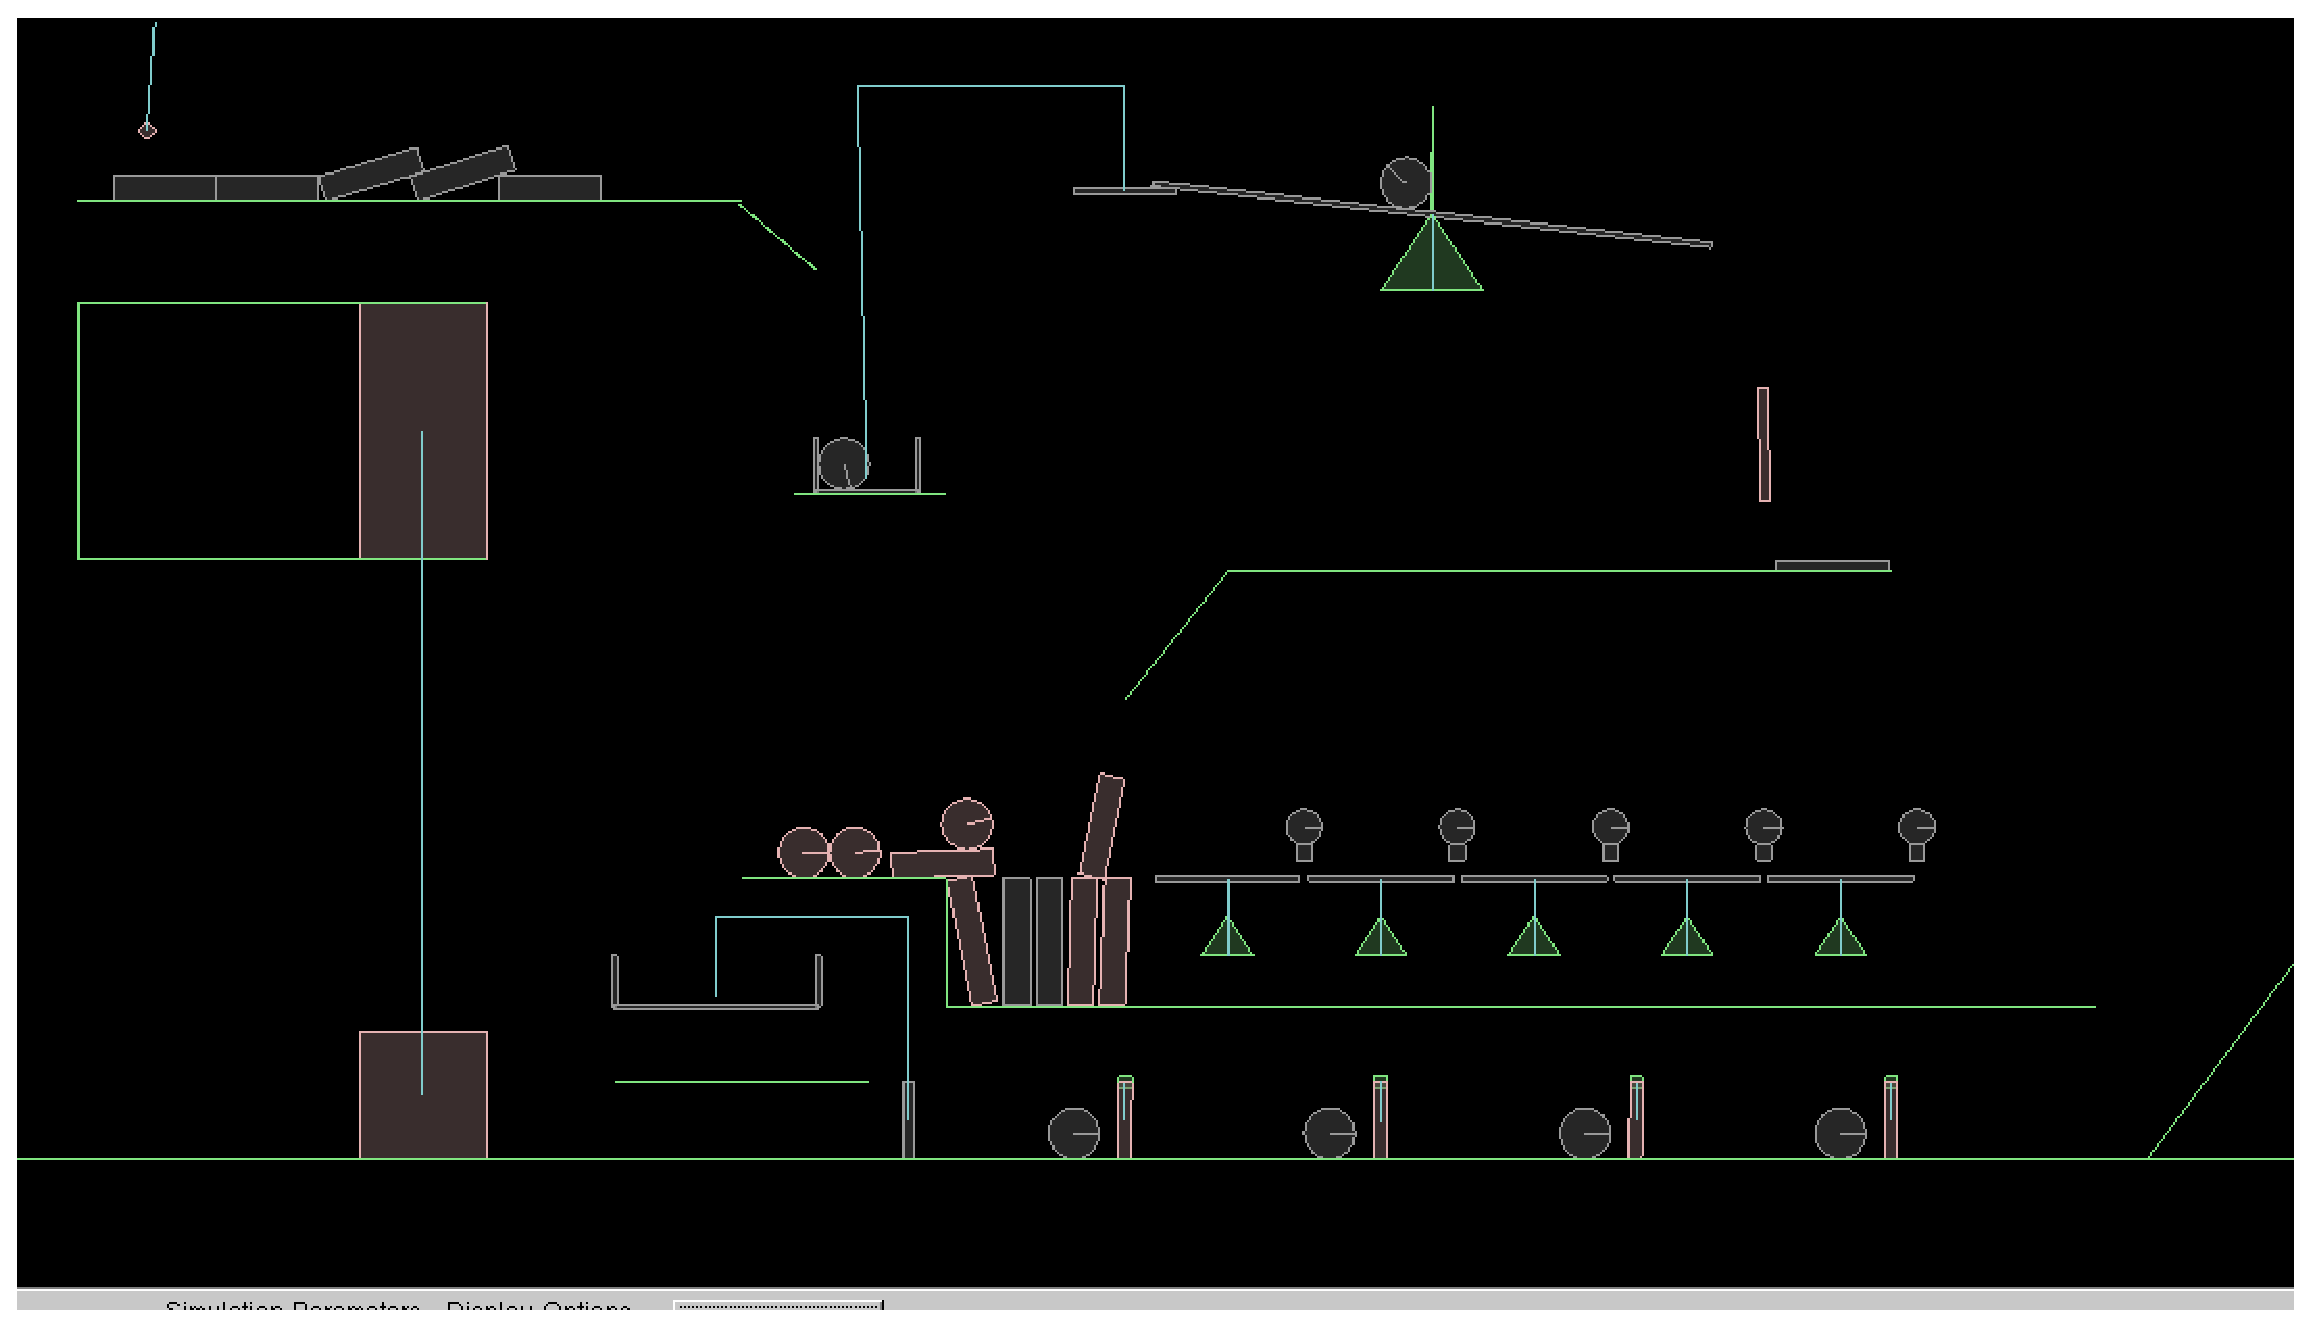
\includegraphics[width=70mm, height=50mm]{state_03.eps}}
\subfloat[Fig. : Stage 4]{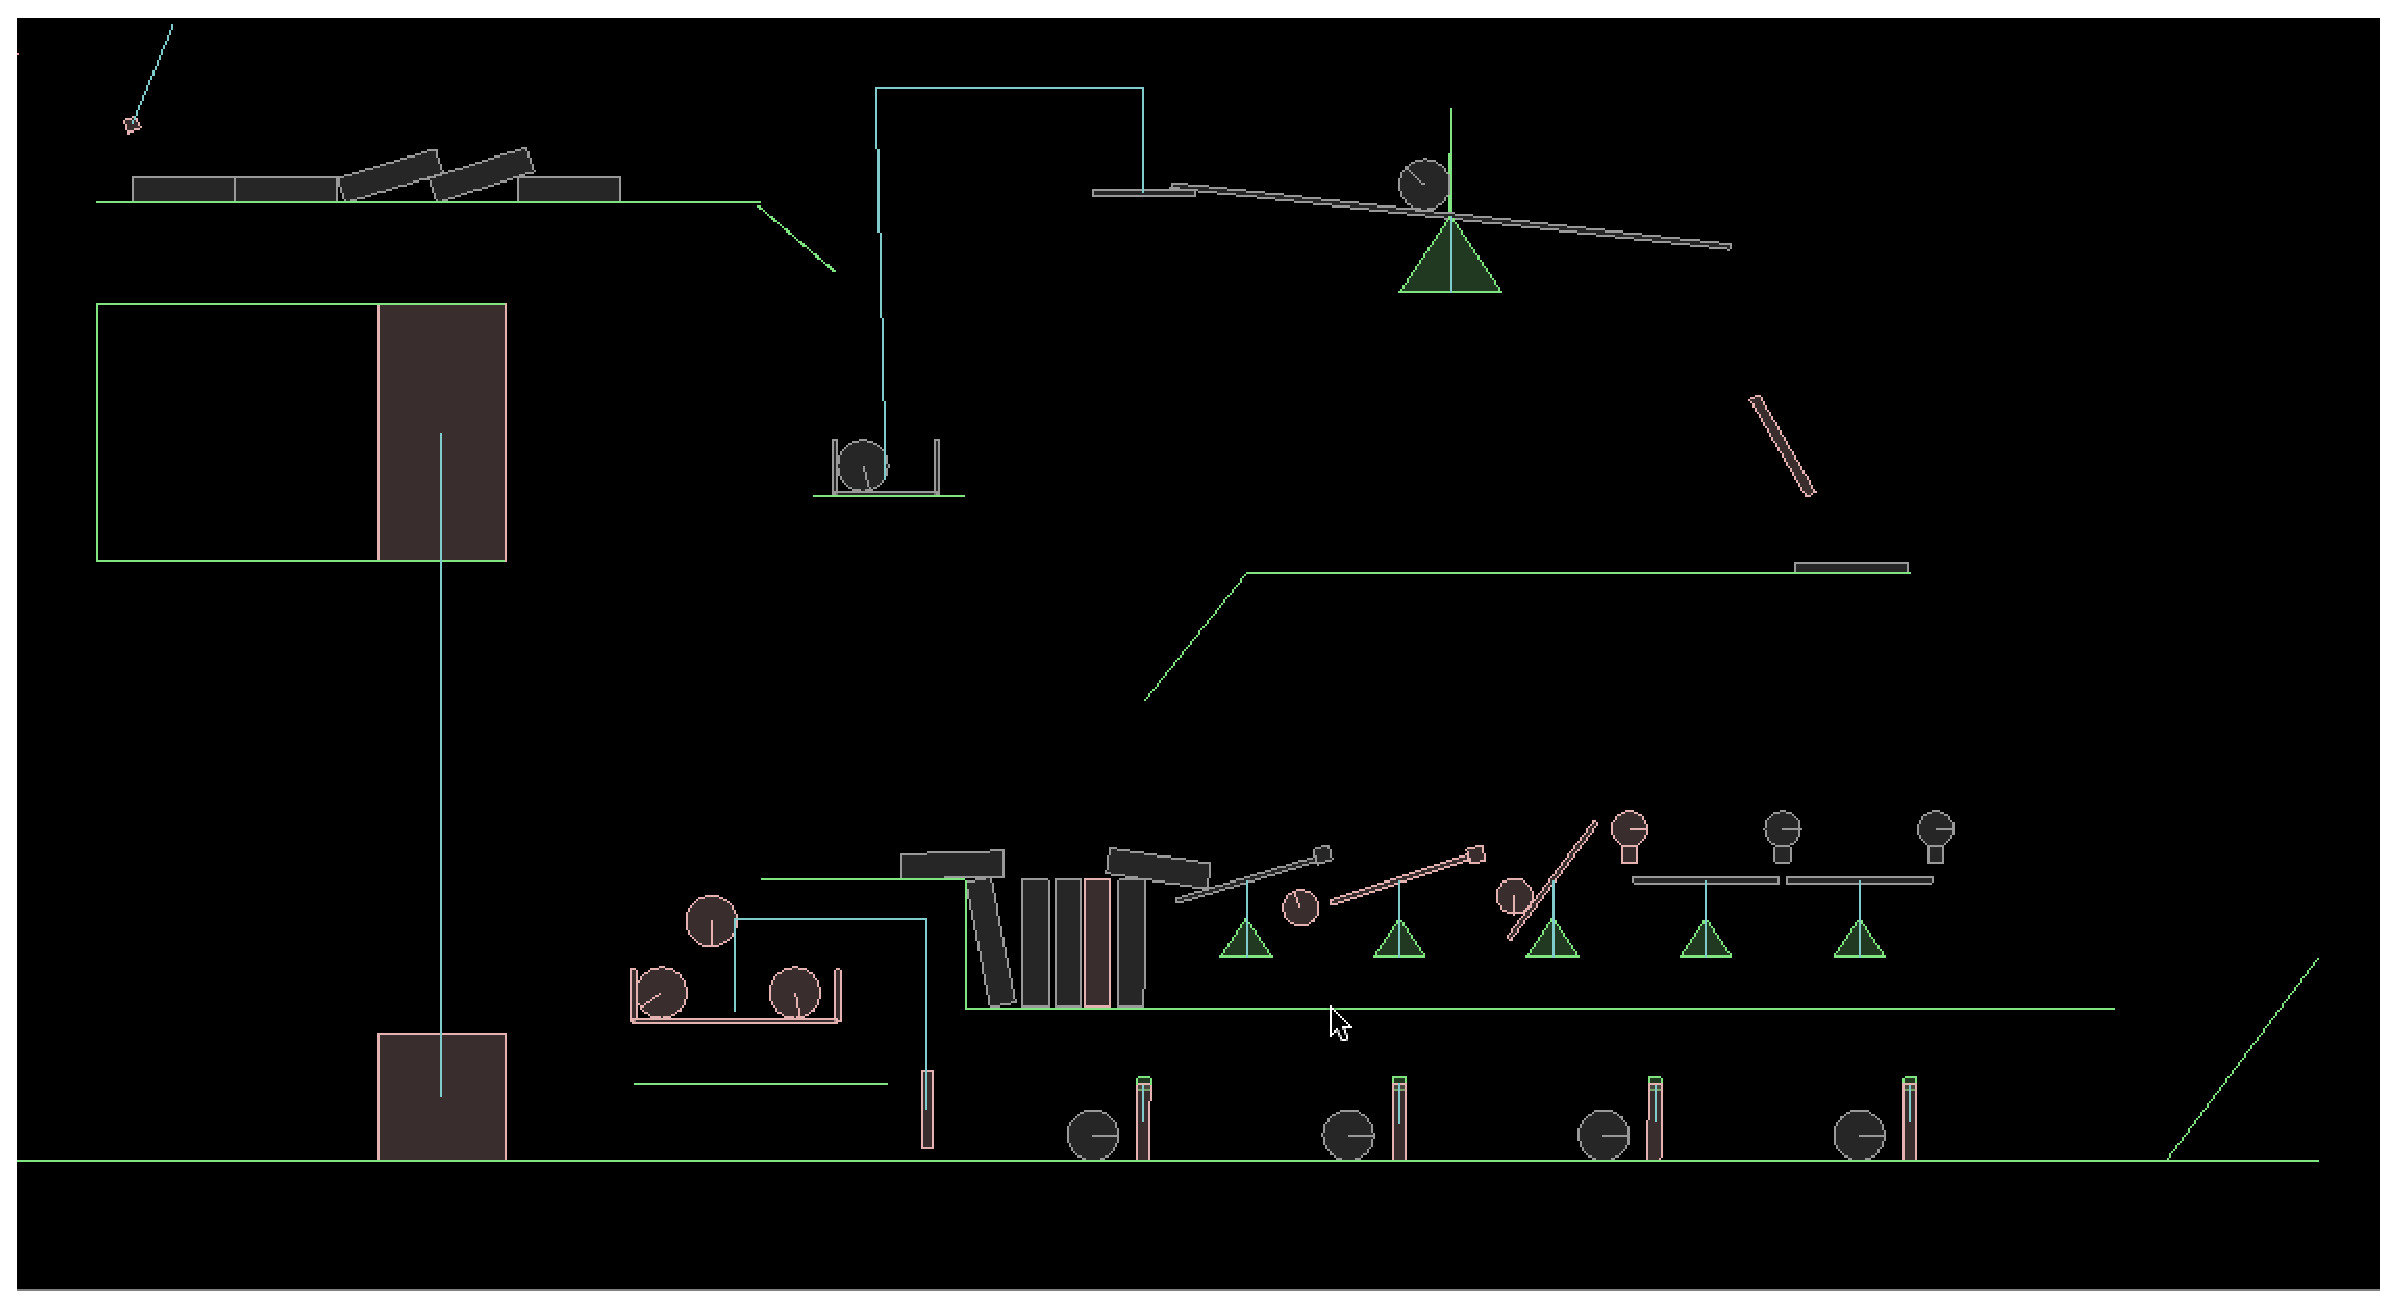
\includegraphics[width=70mm, height=50mm]{state_04.eps}}\\
\subfloat[Fig. : Stage 5]{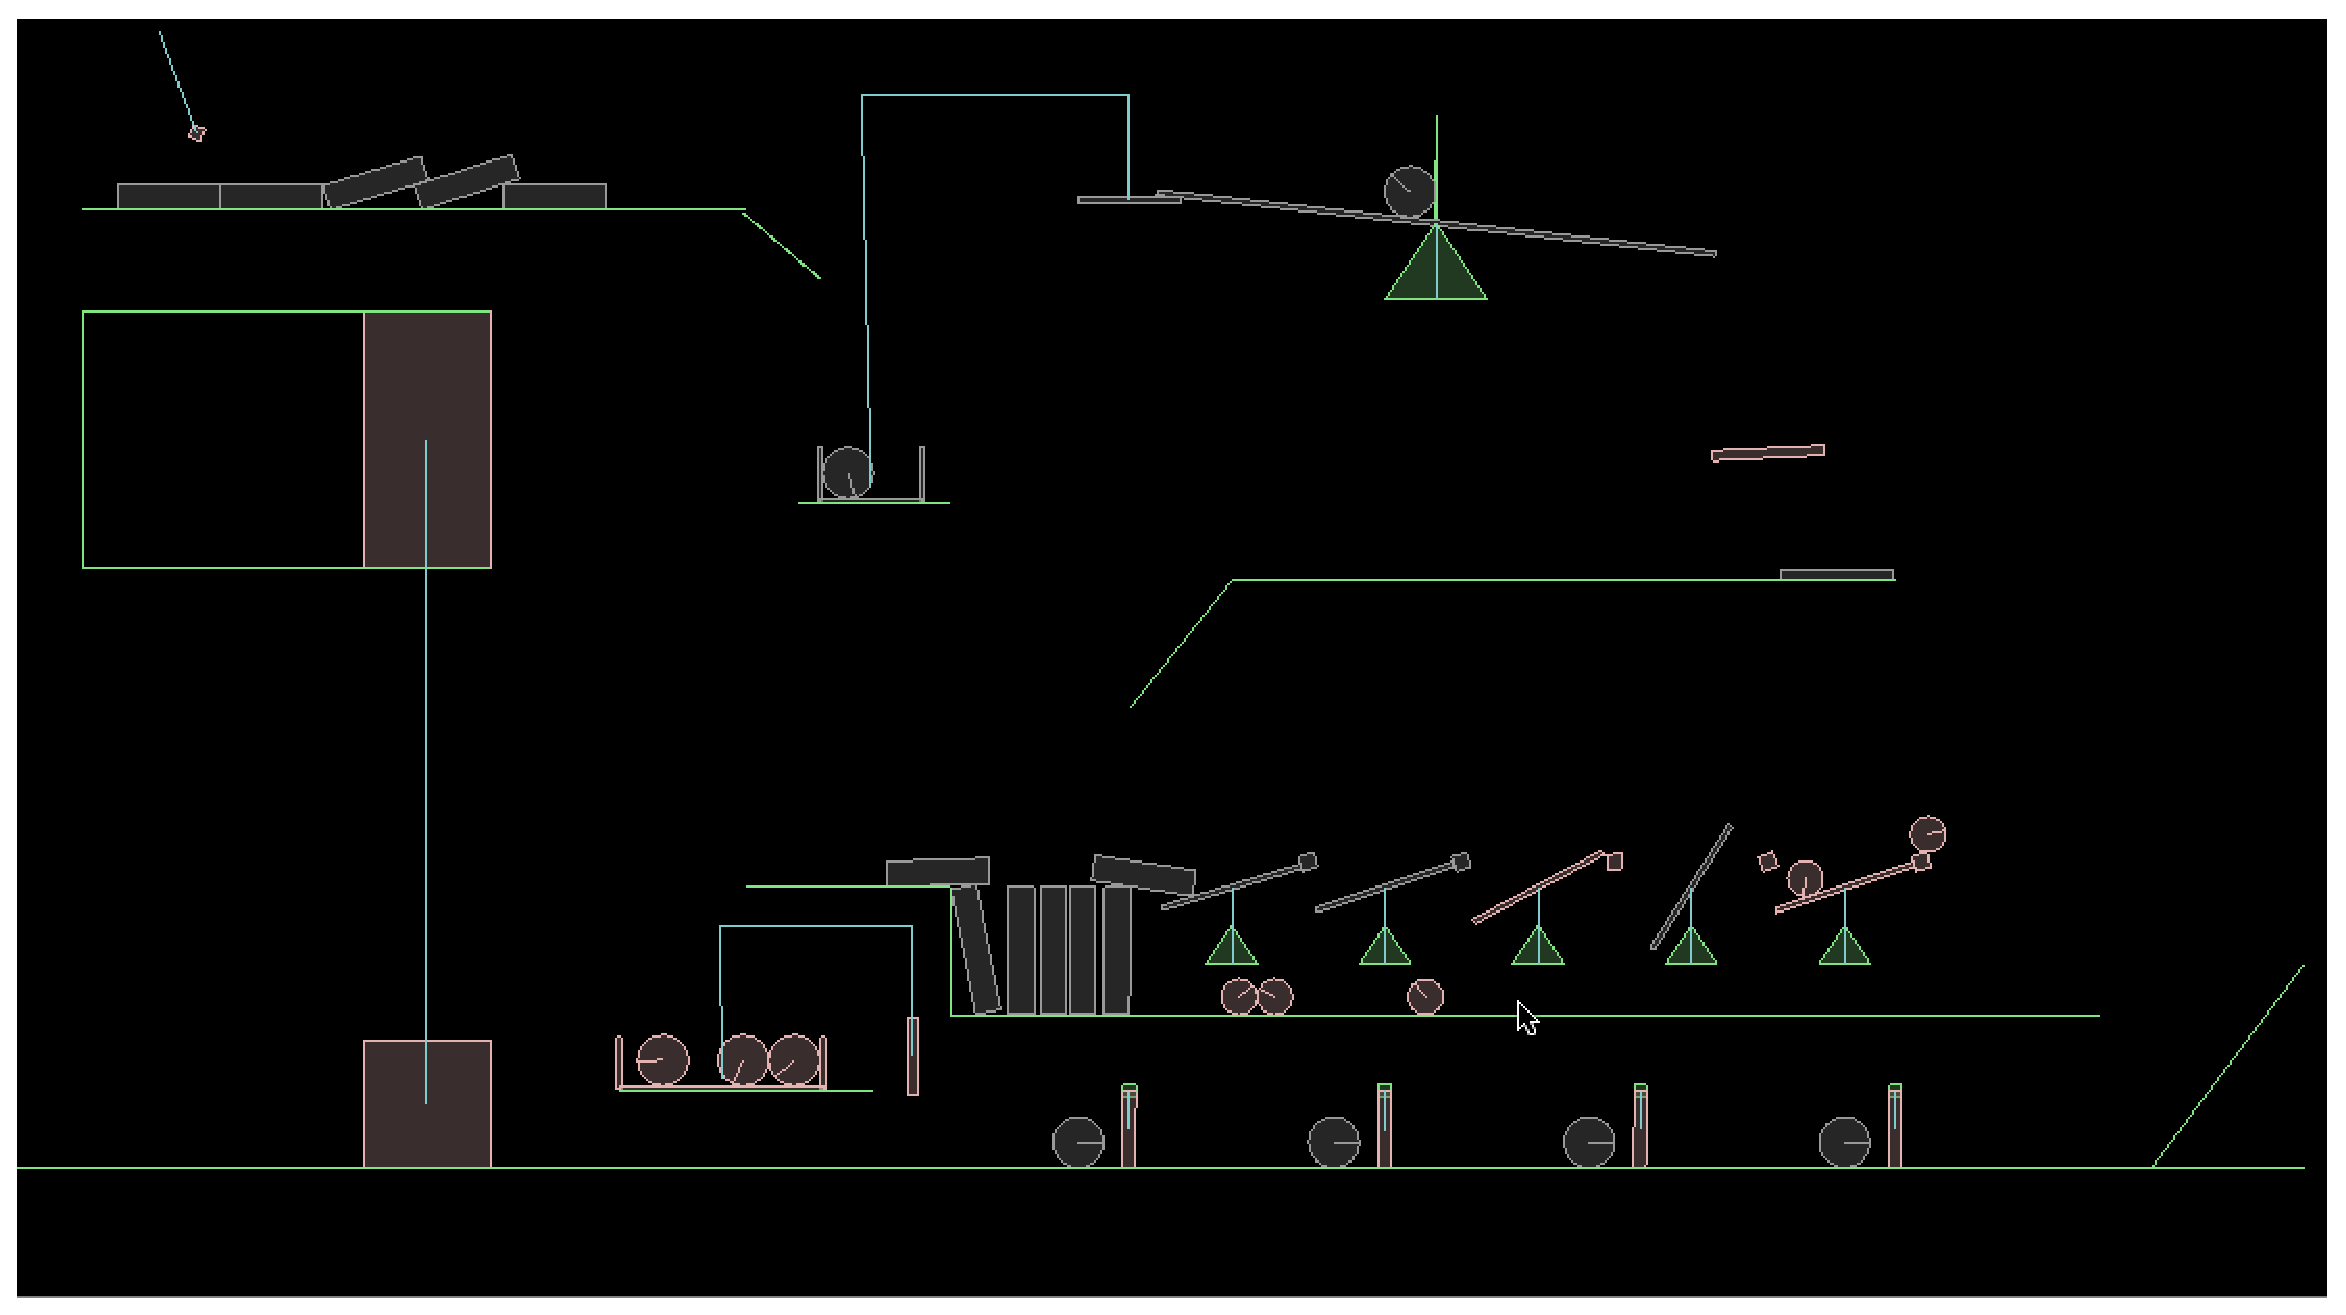
\includegraphics[width=70mm, height=50mm]{state_05.eps}}
\subfloat[Fig. : Stage 6]{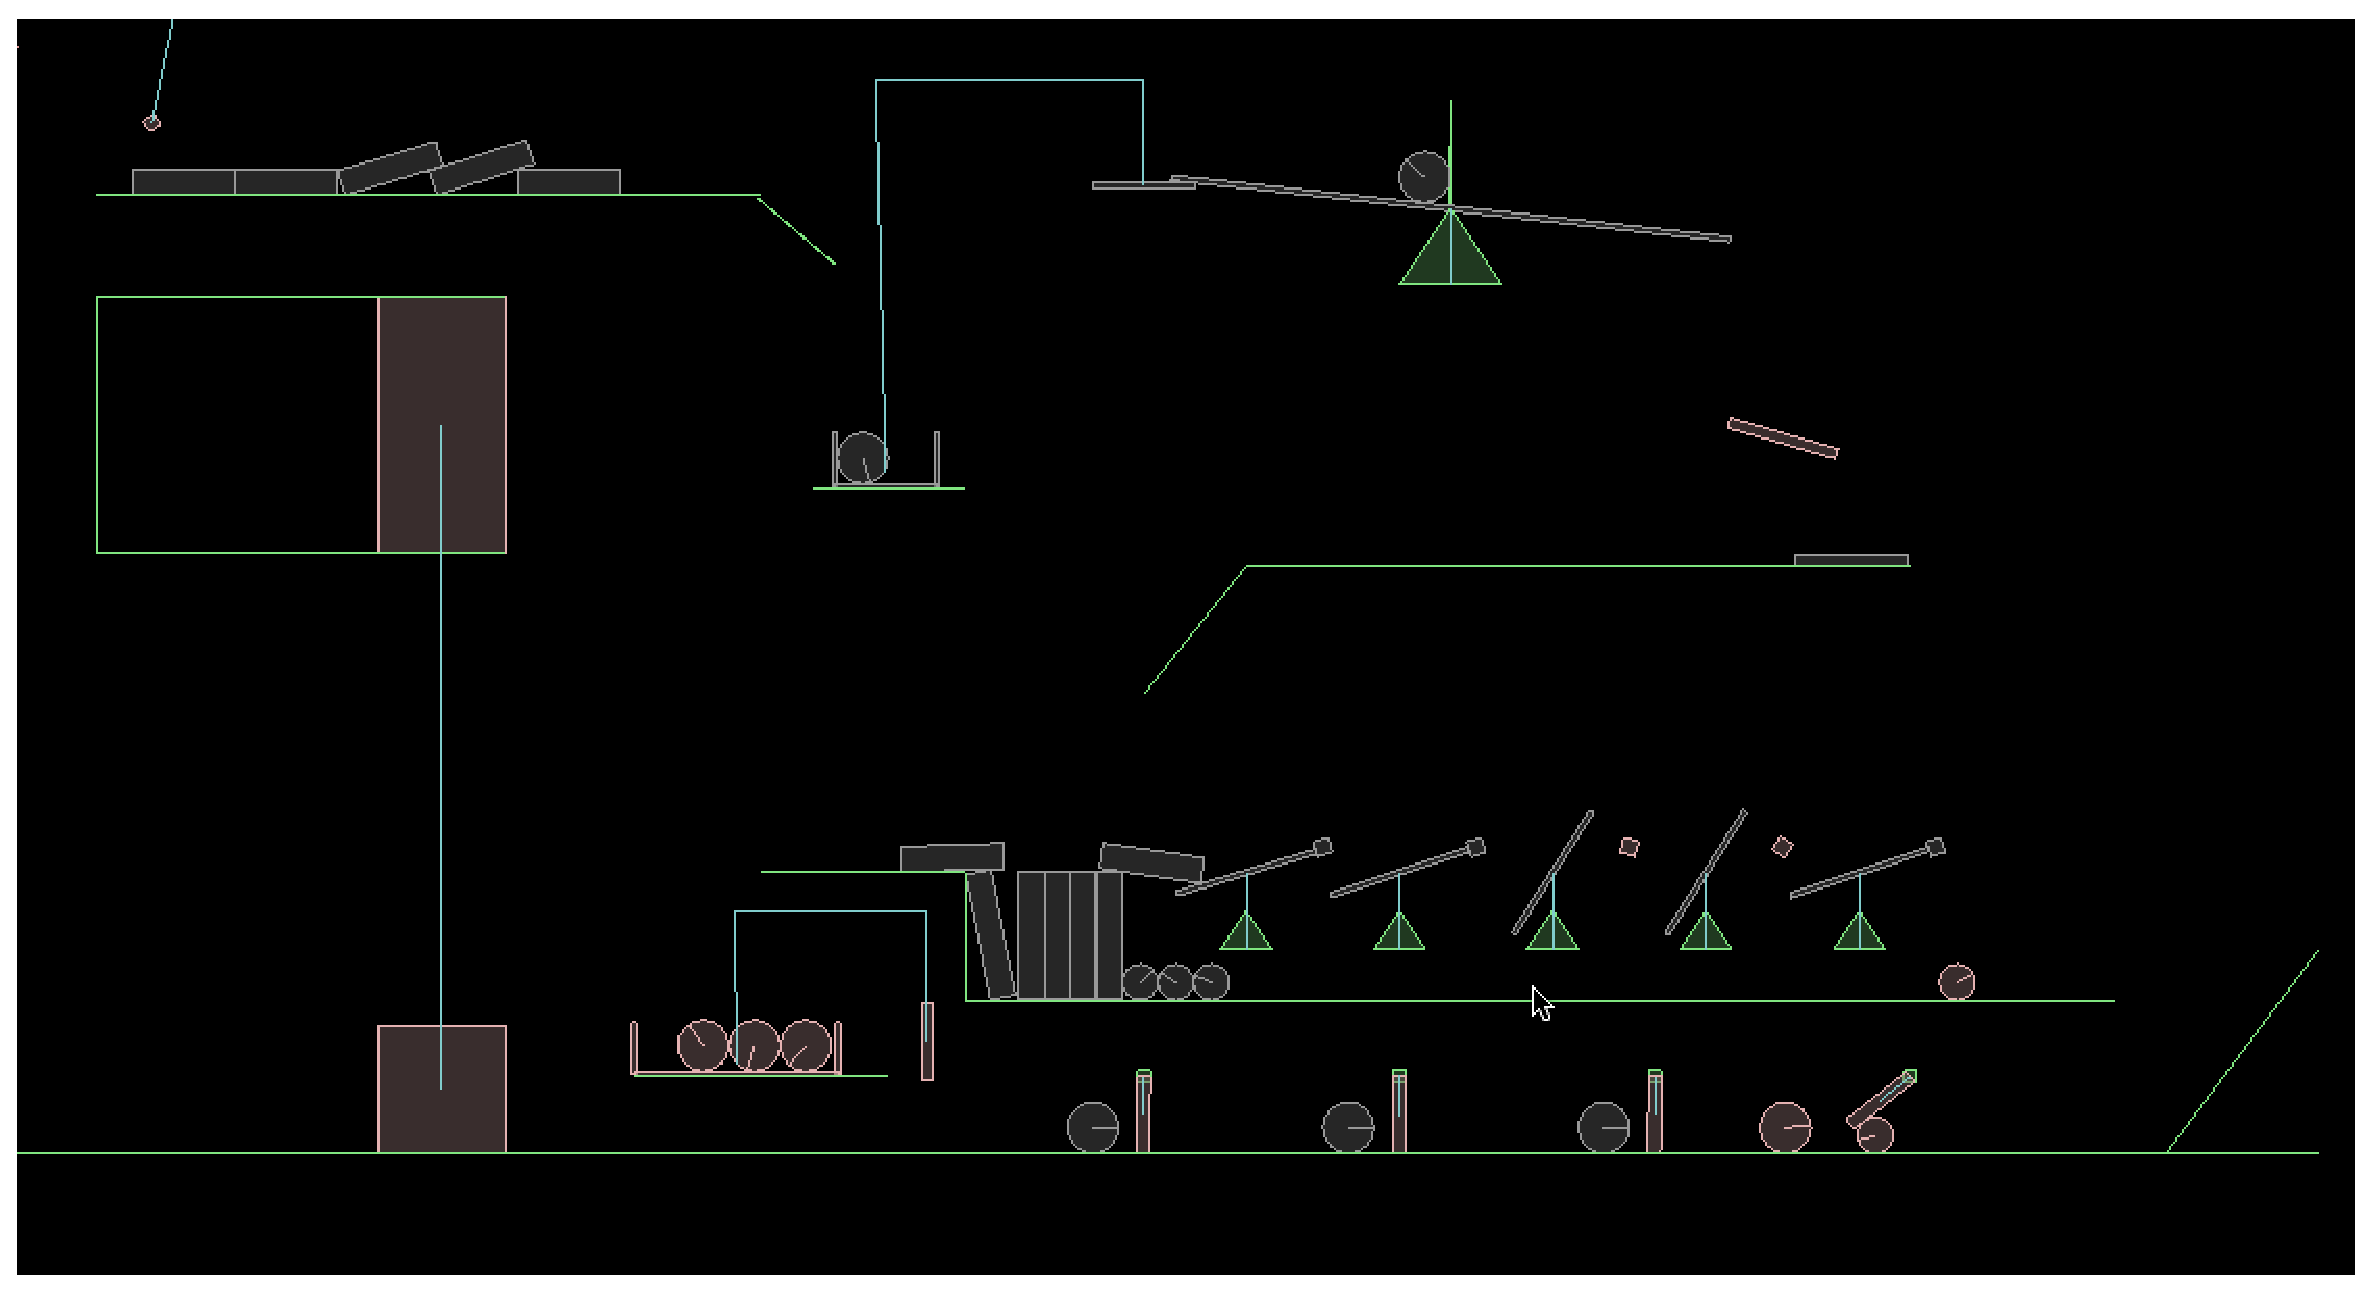
\includegraphics[width=70mm, height=50mm]{state_06.eps}}\\
\subfloat[Fig. : Stage 7]{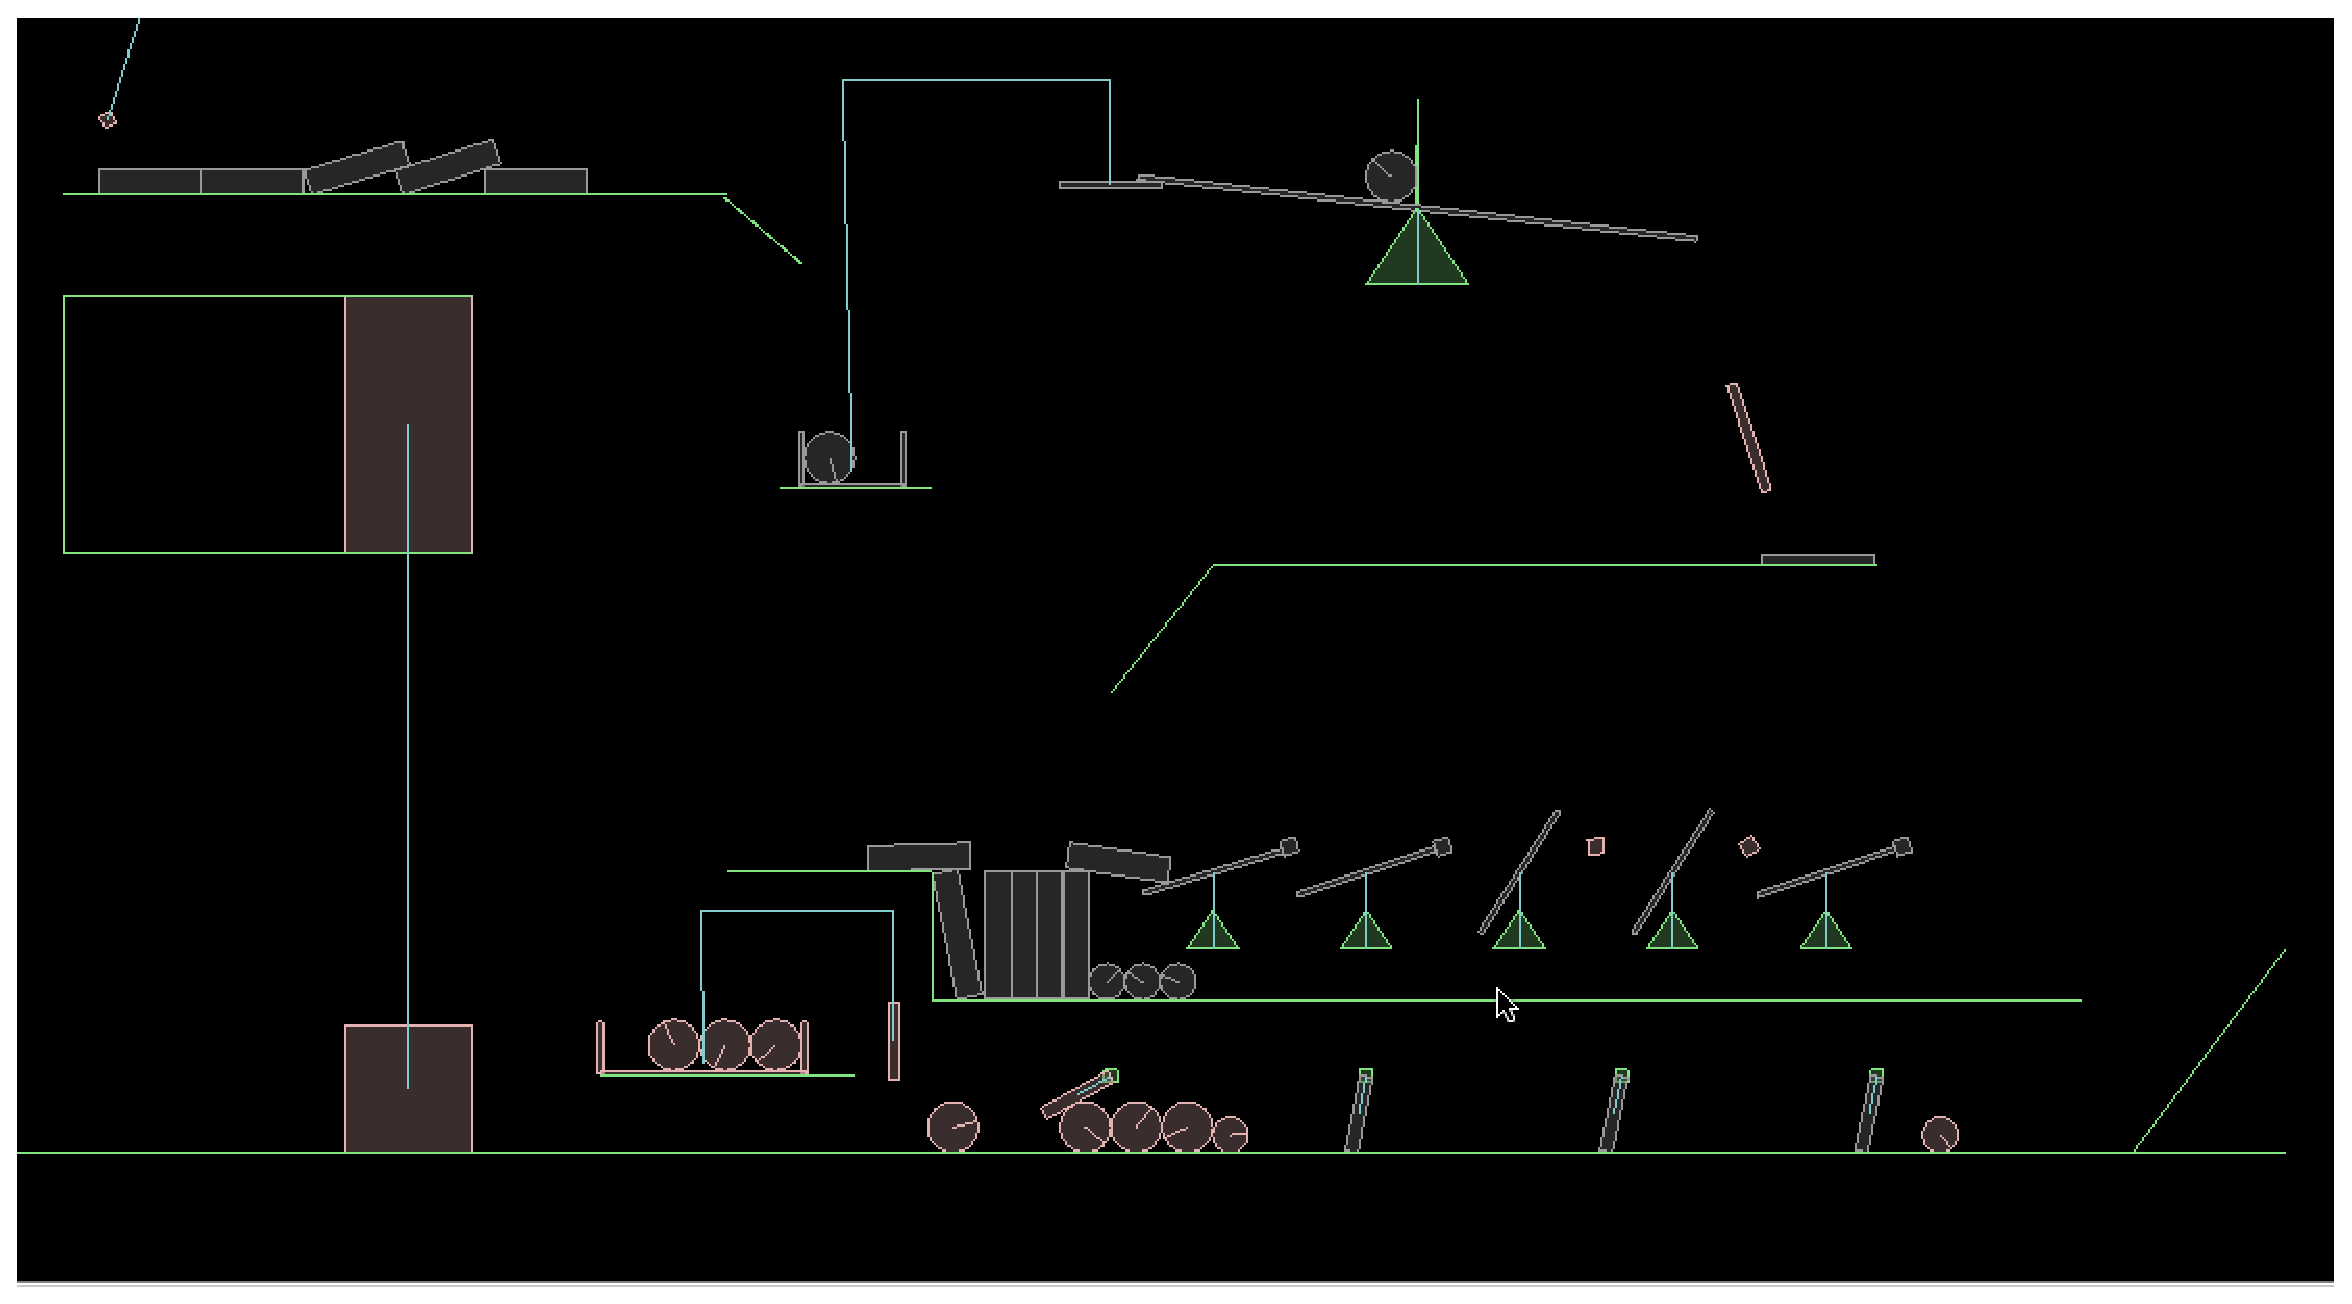
\includegraphics[width=70mm, height=50mm]{state_07.eps}}
\subfloat[Fig. : Stage 8]{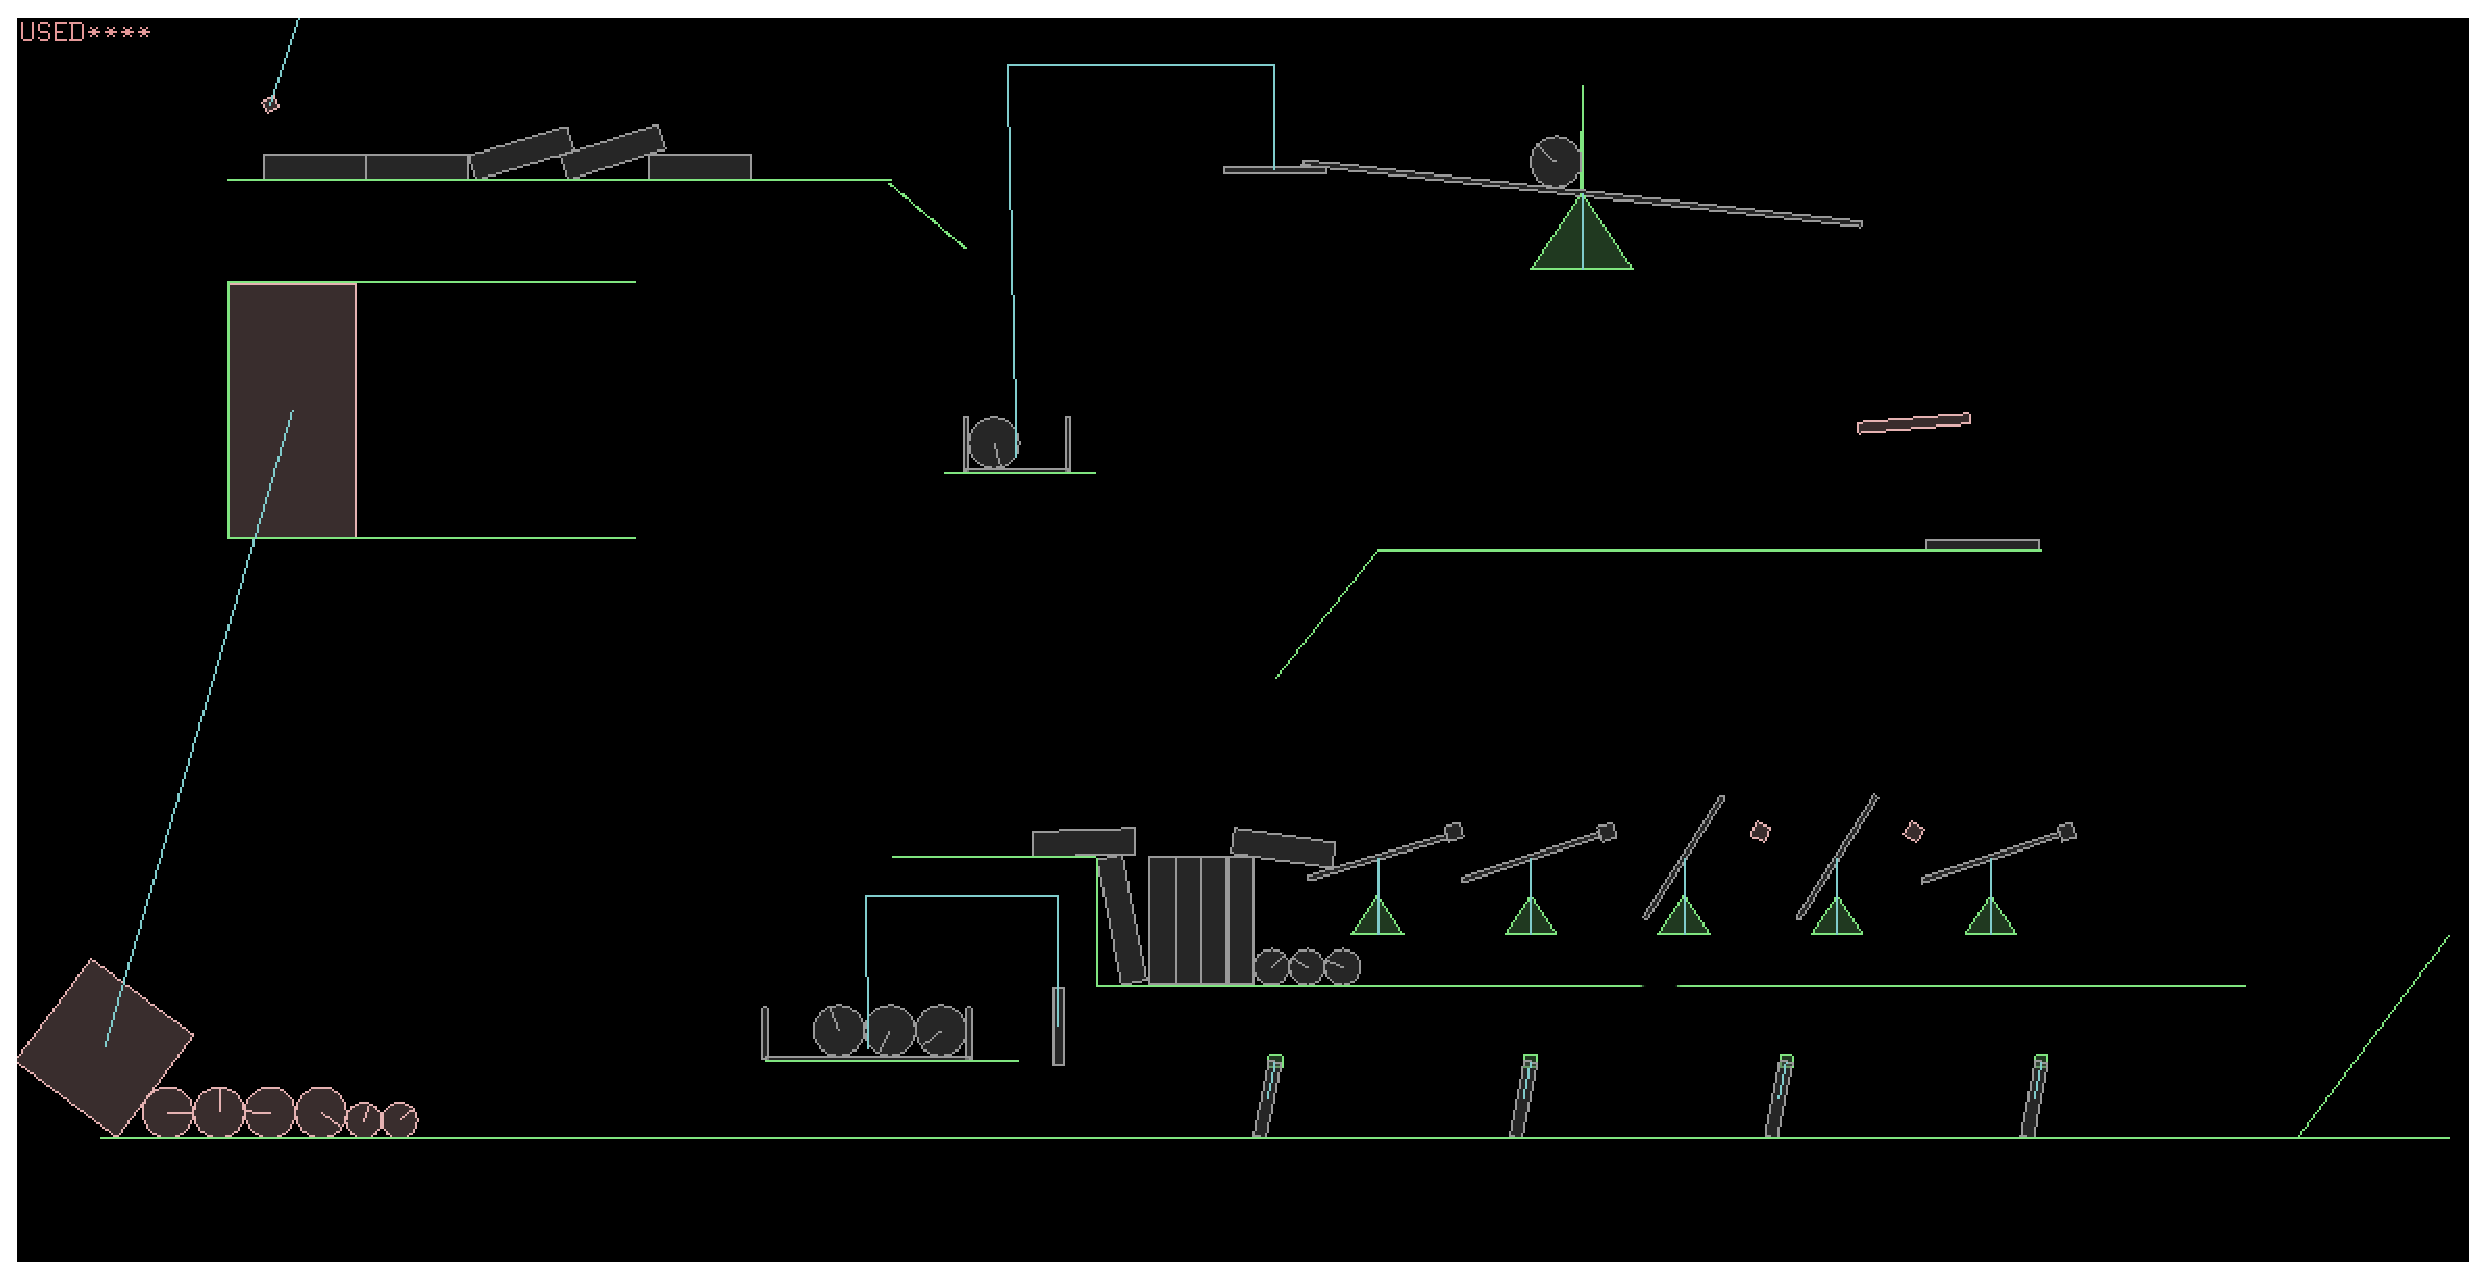
\includegraphics[width=70mm, height=50mm]{state_08.eps}}\\
\caption{The States}
\label{Fig. : Stages of the Simulation}
\end{figure}

\end{document}
